
% \floatname{algorithm}{Table}

\newtheorem{lemma}{Lemma}


\chapter{Efficient elasticity for character skinning with contact and collisions}\label{chap:elasticity}
%\begin{figure}[!ht]
%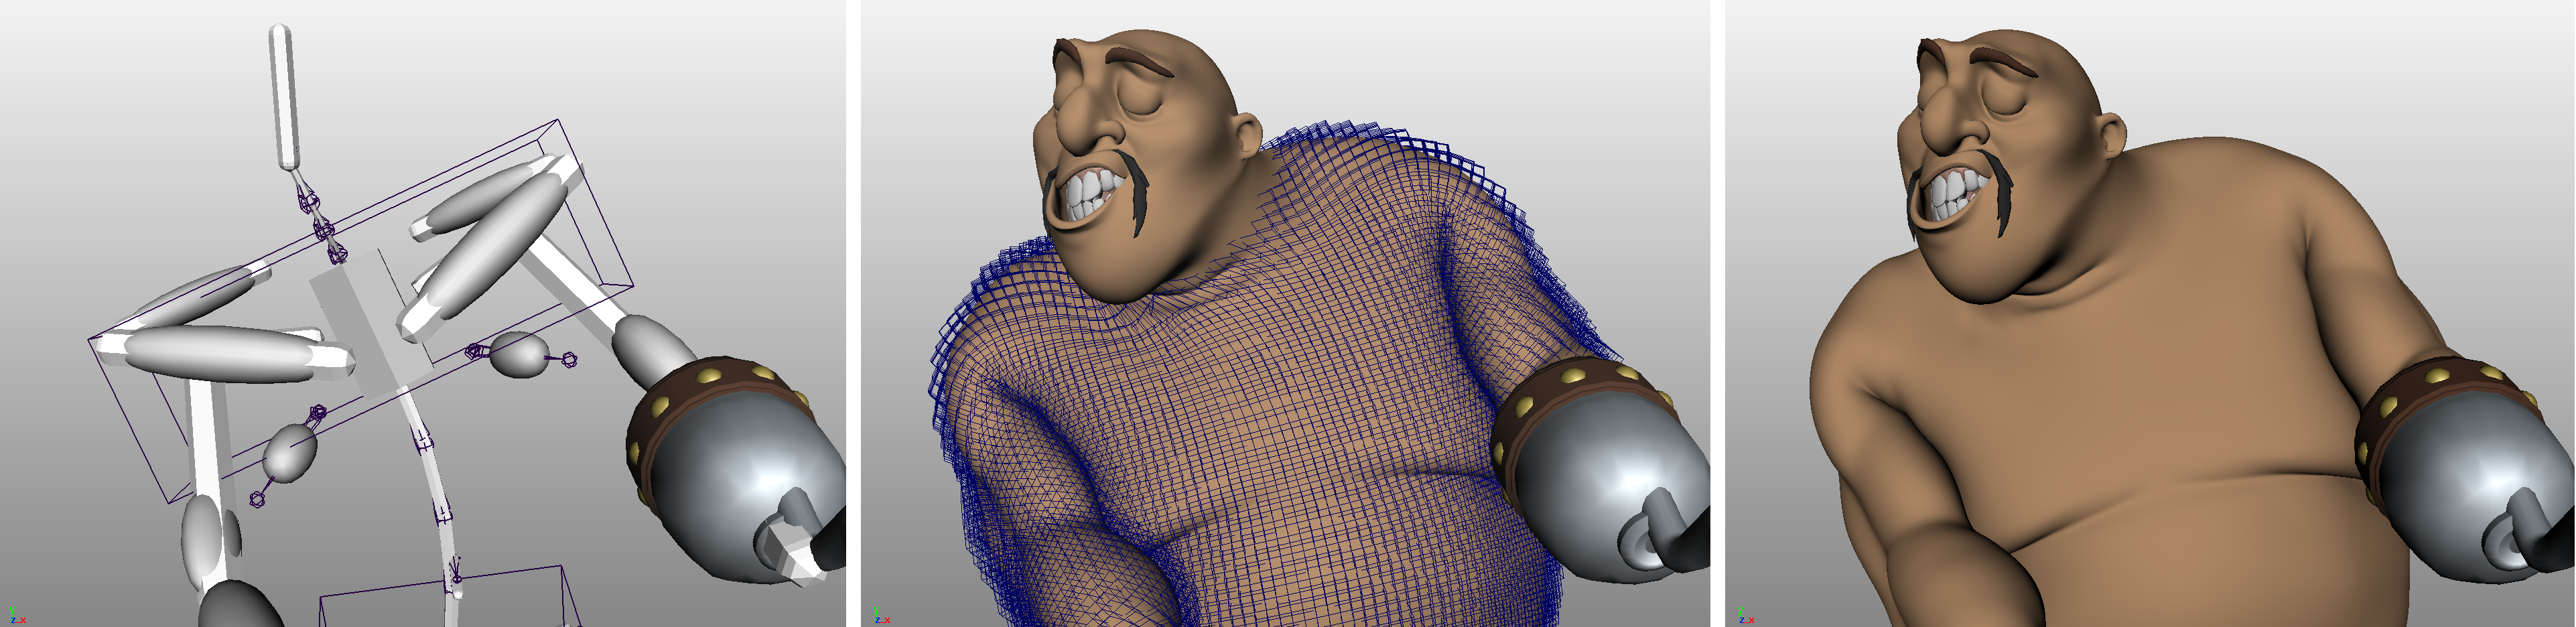
\includegraphics[width=\linewidth]{elasticity/figures/teaser3}
%  \caption{Our method takes a geometric internal skeleton (left) and a source
%    surface mesh (not pictured) as input. Based on a hexahedral lattice (center)
%    it then simulates a deformed surface (right) obeying self-collision and volumetric
%    elasticity. The example shown here has 106,567 cells and simulates at 5.5
%    seconds per frame.}
%\end{figure}
%
%\section{Introduction}
%\label{sec:intro}
%% Existing options
%Creating appealing characters is essential for modern feature animation. One challenging aspect is the production of life-like deformations for soft tissues comprising both humans and animals. In order to provide the necessary control and performance for an animator, such deformations are typically computed using a skinning technique and/or an example based interpolation method. On the other hand, physical simulation of flesh-like material is usually avoided or relegated to an offline process due to its high computational cost. However, simulations create a range of very desirable effects, like squash-and-stretch and contact deformations. The latter is especially important as it can guarantee pinch-free geometry for subsequent simulations like cloth and hair. 

%With time, artists can compensate for the lack of available interactive simulation by tweaking procedural models. Unfortunately, this requires a large amount of effort (potentially weeks per character), so as a consequence the difference in quality between primary and secondary characters can be quite large with existing techniques.

% We want sim to work better
Although the benefits of solving the equations of the underlying physical laws for character deformation are clear, computational methods are traditionally far too slow to accommodate the rapid interaction demanded by animators. Many simplified approaches to physical simulation can satisfy interactivity demands, but any such approach must provide all of the following functionality to be useful in production: (1) robustness to large deformation, (2) support for high-resolution geometric detail, (3) fast and accurate collision response (both self and external objects). Ideally, for rigging, it should also provide (4) path independent deformations determined completely by a kinematic skeleton. However, this may not be possible since contact deformations in general depend on the path taken to the colliding state.

% Instability in the presence of large deformation is a notoriously common problem in Lagrangian simulation of elasticity, however it is unacceptable in a production environment and must therefore be removed by some means. Computational cost for physics based models increases with spatial resolution. A common acceleration is to simply reduce the complexity of the computation model to a few thousand degrees of freedom. Unfortunately, this does not provide the same range of deformations achievable with procedural methods and is therefore inferior in as an animation tool. Perhaps the most significant deficiency of procedural models is the inability to resolve collision/contact phenomena. 

% confounding aspect of skinning procedures is self and external object collision. The inherent inability of procedural models to resolve collision/contact phenomena is the major motivation for simulation based techniques. Any simplified model that does not robustly and interactively resolve collision phenomena is therefore significantly lacking. Finally, for skeleton driven characters, the deformation of the skin and soft tissues must be completely determined by the kinematics of the rig. This is only achievable with a quasistatic assumption for the governing equations of hyperelasticity. However, these equations are non-linear and indefinite and therefore comparatively difficult to solve.

We present a novel algorithmic framework for the simulation of hyperelastic soft tissues that drastically improves each aspect discussed above compared to existing techniques. Our approach is robust to large deformation (even inverted configurations) and extremely stable by virtue of careful treatment of linearization. We present a new multigrid approach to efficiently support hundreds of thousands of degrees of freedom (rather than the few thousands typical of existing techniques) in a production environment. Furthermore, these performance and robustness improvements are guaranteed in the presence of both collision and quasistatic/implicit time stepping techniques. The result is a significant advance in the applicability of hyperelastic simulation to skeleton driven character skinning. We demonstrate the impact of these advances in a complete production system for physics-based skinning of skeletally driven characters. 

%% theoretical contributions
%At the theoretical level, we present a novel discretization of co-rotational
%linear elasticity. This discretization is based on a hexahedral grid, and by
%analyzing the properties of the co-rotational formulation we minimize both the
%number of quadrature points and polar decompositions required. The linearization
%in co-rotational elasticity is often indefinite, but we guarantee stability in
%the presence of both indefiniteness and inversions. Finally, we show how to
%solve the problem efficiently with a multigrid approach.

%% implemention contributions

%Targeting practical utilization requires the implementation to be as efficient as possible. Our discretization is designed to be cache and streaming friendly and we balance the tradeoff between computation and memory bandwidth. The discretization also allows us to compute just a single SVD per cell as opposed to 8 SVDs for a standard Gauss quadrature rule. To further accelerate the computations we present a new branch-free algorithm for computing SVDs. This by itself is 40 times faster than what has previously been reported \cite{Rivers:2007:FFL,Kopp08}. In practice we have implemented and tested our entire system both on multithreaded CPUs as well as in the CUDA GPU framework. Unlike many efforts that focus on performance, we handle collision, self-collision, and soft constraints, all of which are essential in a production environment.

%% roadmap
%\todo{This needs work} The rest of the paper proceeds as follows:
%In section~\ref{sec:elasticity} we describe our elastic model followed by
%section~\ref{sec:constraints} which discusses constraints and collisions.  Then
%in section~\ref{sec:multigrid} we show how the equations are efficiently solved
%with multigrid.  Implementation details concerning GPU/CPU and performance are
%discussed in section~\ref{sec:implementation}. Finally we show our method
%applied to actual production examples in section~\ref{sec:results} and 
%we discuss the technique in section~\ref{sec:discussion}.

\section{Related work}
\label{sec:relatedwork}



% skinning

Skeleton driven skin deformation was first introduced by \cite{Magnenat-Thalmann89}. Since then such techniques have been used extensively, especially the ``linear blend skinning'' technique (aka.\ ``skeleton subspace deformation'' (SSD) or ``enveloping''). However, the limitations of such techniques are well-known and have been the topic of numerous papers \cite{Wang02,Merry06,Kavan08}. Despite improvements, skinning remains, for the most part purely kinematic. It has proven very difficult to get more accurate, physically based deformations (e.g., from self-collisions and contact with other objects). Rather, such phenomena are typically created through a variety of example based approaches \cite{Lewis00,Sloan01}. Although very fast computationally, example based methods often require extreme amounts of user input, especially for contact and collision.

% elasticity based approaches
Simulation recently enabled significant advances to character realism in \cite{Irving:2008:SDF} and \cite{clutterbuck:2010:avatar}, albeit with the luxury of extreme computation time. Nevertheless these approaches demonstrated the promise of simulation. Many techniques reduce the accuracy of the elasticity model to help improve performance and interactivity. \cite{Waters90,Chadwick89} first demonstrated the effectiveness of comparatively simple mass/spring based approaches. \cite{Sueda:2008} add interesting anatomic detail using the tendons and bones in the hand, but use simple surface-based skin. \cite{Kry02} use principle component analysis of off-line elasticity simulation to provide interactive physically based SSD. \cite{capell:2005:pb,Capell:2002:ISD:566570.566622,Galopo07} used a skeleton based local rotational model of simple linear elasticity. \cite{Muller:2005:MDB} introduced shape matching, a technique that uses quadratic modal elements defined per lattice cell, allowing realtime albeit less accurate deformations. \cite{Rivers:2007:FFL} extended the accuracy of this
method while maintaining high performance with a fast SVD. Warped stiffness approaches \cite{Muller:2002:SRD,Muller:2004:IVM} are a more general example of the techniques developed by Cappel et al.\ and use an inexact force differential to yield easily solvable symmetric positive definite (SPD) linearizations. However, \cite{Chao:2010:SGM} recently demonstrated the importance of a more accurate approximation to rotational force differentials lacking in warped stiffness approaches. We  illustrate this important robustness limitation of the warped stiffness approximation in figure~\ref{fig:warpedstiff}. The instability of the method effectively precludes its use in skinning applications. Unfortunately, the more accurate linearizations  yield indefinite systems and thus require more expensive linear algebra techniques (e.g., GMRES). However we demonstrate a solution procedure in the present work that rivals the efficiency available to warped stiffness, but without the robustness difficulties.

% multigrid

Typically elastic simulation requires the solution of large sparse systems. Conjugate gradients is a popular method for solving such systems by virtue of simplicity and low-memory overhead; however, it is plagued by slow convergence (especially with high resolution models). Multigrid techniques potentially avoid these convergence issues, but can be costly to derive for problems over irregular domains. \cite{Zhu:2010:EMM} developed a multigrid approach that achieves nearly optimal convergence properties for incompressible materials in irregular domains. However, their technique for corotational elasticity uses a pseudo-Newton iteration that does not guarantee convergence on the large deformations typical in skeleton driven animation. \cite{Dick:2011:CUDAFEM,Georgii06,Wu04} also examine multigrid methods for rapidly solving the equations of corotational elasticity. However these techniques are based on the warped stiffness approximation to corotational force differentials and demonstrate similar convergence issues as Zhu et al. Multigrid has also been shown to provide excellent parallel performance (e.g., on the GPU in \cite{Dick:2011:CUDAFEM} and on the CPU in \cite{Zhu:2010:EMM}). Our multigrid approach is the first to robustly provide near-interactive performance for non-linear elasticity models with hundreds of thousands of degrees of freedom.


\section{Elasticity and discretization}
\label{sec:elasticity}
The previously discussed demand for high-resolution simulation with optimal
performance and robustness motivated the development of our novel co-rotational
elasticity discretization. Following \cite{Chao:2010:SGM}, we use an accurate
treatment of force derivatives to yield a more robust solver than the
simplified warped-stiffness techniques. We show that these careful
linearizations can be done both cheaply and simply and are essential for our desired
robustness and efficiency. We perform our discretization over a
uniform hexahedral lattice  (rather than an unstructured tetrahedral one) to
facilitate performance on modern hardware. Although standard methods for
hexahedra require 8 point Gauss quadrature per cell for stability, we develop a
much more efficient one-point quadrature discretization
(section~\ref{sec:stabilization}).

\subsection{Fundamentals}
\label{sec:fundamentals}

We represent the deformation of a 3D elastic body by a function $\vec{\phi}:\Omega\rightarrow\mathbf{R}^3$, which maps a material point
$\vec{X}$ to a deformed world-space point $\vec{x}$ so $\vec{x}=\vec{\phi}(\vec{X})$. Subsequently, we use $\vec{x}$ and $\vec{\phi}$ interchangeably,
i.e.\ we identify $\vec{x}(\vec{X})\equiv\vec{\phi}(\vec{X})$. For hyperelastic
materials in general, the response can be computed based on the deformation energy:
\begin{equation}
E=\int_\Omega\Psi(\vec{X},\mathbf{F}(\vec{X}))d\vec{X}
\label{eqn_energy_integral}
\end{equation}
For simplicity we will here consider the energy density $\Psi$ as a function of the
deformation gradient $F_{ij}=\partial\phi_i/\partial\vec{X}_j$. Specifically for
corotational elasticity we have
%For typical materials, the elastic energy density $\Psi$ appearing in equation (\ref{eqn_energy_integral}) is a function of the Jacobian of $\phi$, also known as the  deformation gradient  
%$\mathbf{F}$ (i.e.\ $F_{ij}=\partial\phi_i/\partial\vec{X}_j$). The additional explicit dependence of $\mathbf{F}$ on the material coordinates $\vec{X}$ allows for inhomogeneous material
%parameters; for simplicity we shall initially focus on homogeneous elasticity where $\Psi$ is purely a function of $\mathbf{F}$. Corotational linear elasticity defines this energy
%density as follows:
\begin{equation}
\Psi=\mu\|\mathbf{F}-\mathbf{R}\|_F^2+\frac{\lambda}{2}\tr^2(\mathbf{R}^T\mathbf{F}-\mathbf{I})
\label{eqn_energy_F}
\end{equation}
where $\mu,\lambda$ are the Lam\'{e} coefficients, and $\mathbf{R}$ is the rotation from the polar decomposition $\mathbf{F}=\mathbf{RS}$.

\subsection{Energy discretization}

We discretize our model domain $\Omega$ into cubic elements $\Omega_e$ of step size $h$ so $\Omega=\cup_e\Omega_e$. The degrees of freedom are world space samples of
$\vec{x}_i=\vec{\phi}(\vec{X}_i)$. The discrete version of
equation~(\ref{eqn_energy_integral}) then becomes a sum of energies from each element $E_e$.  Using just a single quadrature point for the voxel center $\vec{p}^c$ gives $E_e \approx h^3\Psi(\mathbf{F}^e)$ where $\mathbf{F}^e\approx\mathbf{F(\vec{p}^c)}$ is computed with central differences about the cell center from averaged faces.
\begin{figure}
\centering
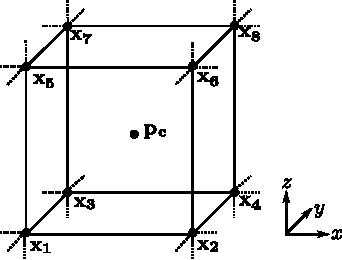
\includegraphics[width=.35\columnwidth]{elasticity/figures/grid.pdf}
\caption{A sample cubic element.}\label{fig:cubic_element}
\end{figure}
 This approximation can be written
\begin{equation}
F_{ij}^e=\sum_kG_{jk}^ex_k^{(i)}
\label{eqn_discrete_gradient}
\end{equation}
where $x_k^{(i)}$ is the $i$-th component of the three-dimensional vector $\vec{x}_k$ (see Figure~\ref{fig:cubic_element}) and we have
a \emph{discrete gradient}
{\small$$
\mathbf{G}^e=
\frac{1}{4h}
\left(
\begin{array}{cccccccc}
-1 &  1 & -1 &  1 & -1 &  1 & -1 &  1 \\
-1 & -1 &  1 &  1 & -1 & -1 &  1 &  1 \\
-1 & -1 & -1 & -1 &  1 &  1 &  1 &  1
\end{array}
\right).
$$}
Finally, we have a means to compute the total energy in terms only of the nodal world positions of our hexahedral lattice.



\begin{figure}[th]
\center{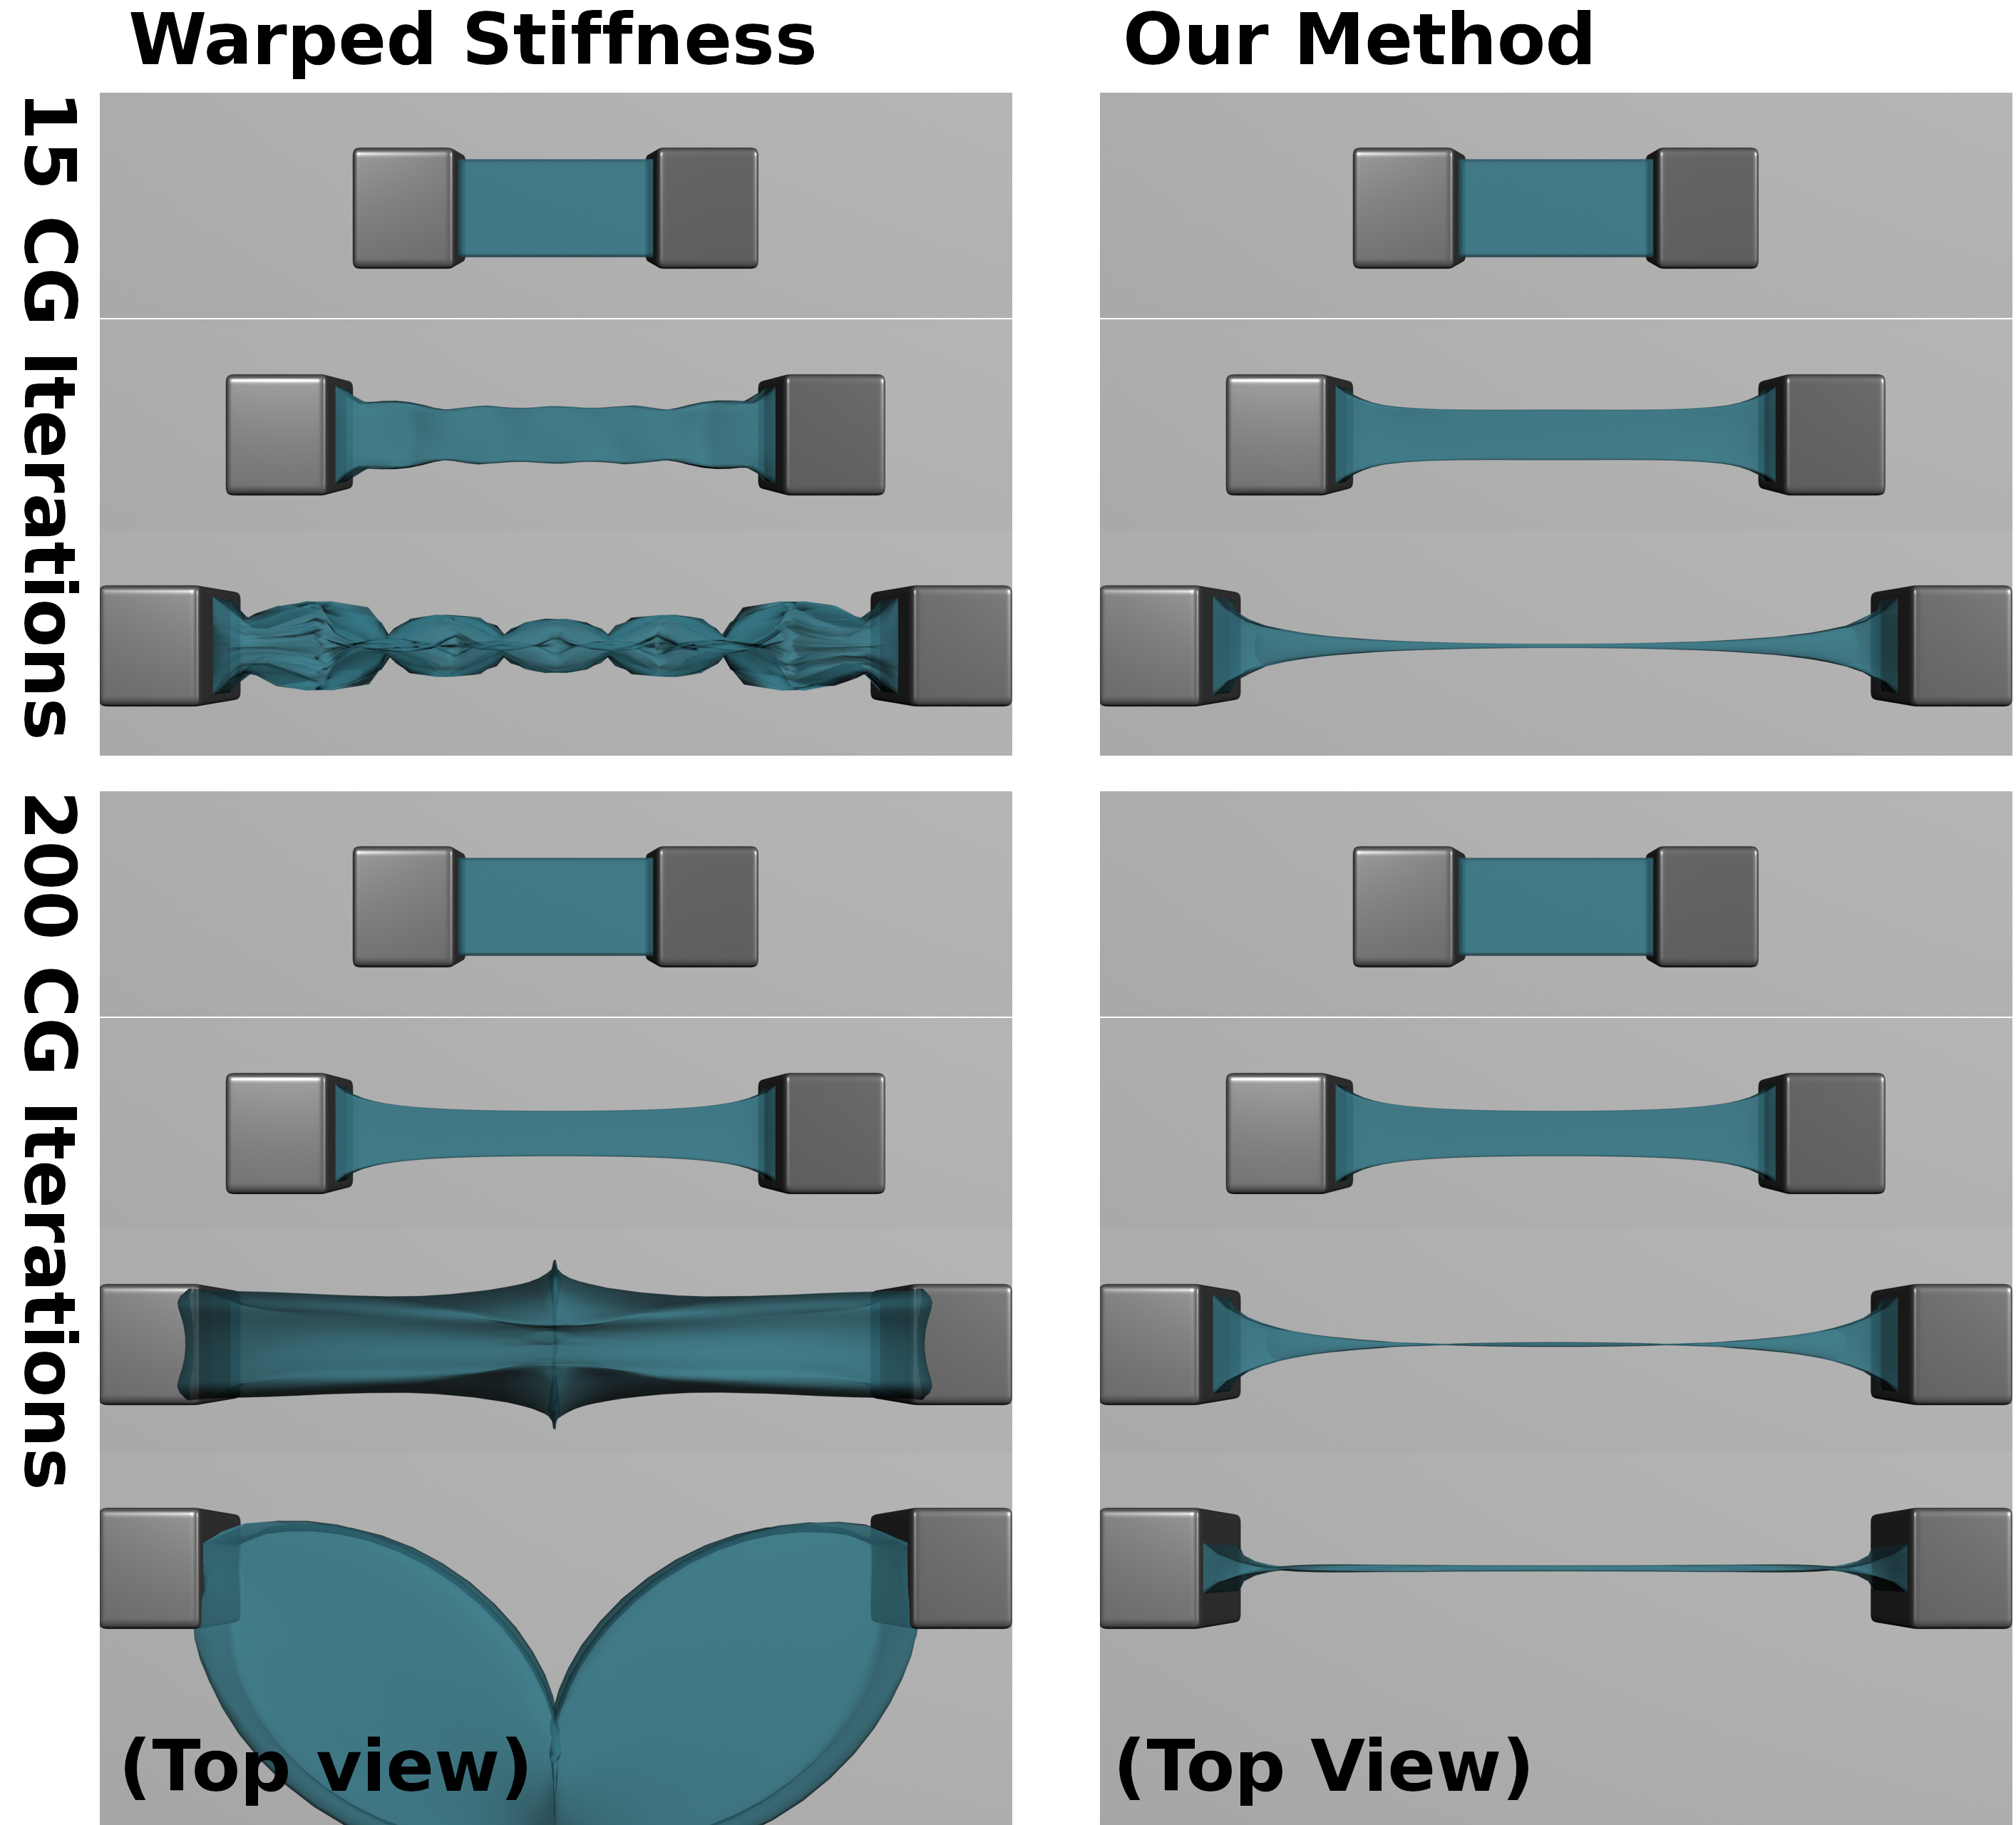
\includegraphics[width=.7\linewidth]{elasticity/figures/warpedcomp}}
\caption{Inexact methods of computing force differentials lead to instabilities
unlike our method}
\label{fig:warpedstiff}
\end{figure}

\subsection{Force and equilibrium}
\label{sec:force}

A discrete force per node can in general be written as
\begin{equation}
\vec{f}_i=-\frac{\partial E}{\partial\vec{x}_i}=\sum_e\left(-\frac{\partial E_e}{\partial\vec{x}_i}\right)=\sum_e\vec{f}_i^e.
\label{eqn_elemental_forces}
\end{equation}
%Intuitively, we identify the quantity $\vec{f}_i^e=-\partial E_e/\partial\vec{x}_i$ in the last equation with the contribution of element $\Omega_e$ to the forces exerted on node
%$\vec{x}_i$.
 Using equation (\ref{eqn_discrete_gradient}) and the fact that $\Psi$ is a function of the deformation gradient alone, a concise expression for each of the components
of $\vec{f}_i^e=(f_i^{(1)},f_i^{(2)},f_i^{(3)})$ (the force contribution to node $i$ from element $e$) is: 
\begin{eqnarray}
f_i^{(j)}\!\!\!&\!\!\!=\!\!\!&\!\!\!-\frac{\partial E_e}{\partial\vec{x}_i^{(j)}}=-V_e\frac{\partial\Psi(\mathbf{F}^e)}{\partial\vec{x}_i^{(j)}}
=
-V_e\sum_{k,l}\left.\frac{\partial\Psi}{\partial F_{kl}}\right|_{\mathbf{F}^e}\frac{\partial F_{kl}^e}{\partial\vec{x}_i^{(j)}} \nonumber \\
\!\!\!&\!\!\!=\!\!\!&\!\!\!
-V_e\sum_{k,l}[\mathbf{P}(\mathbf{F}^e)]_{kl}G_{li}^e\delta_{jk}
=
-V_e\sum_l[\mathbf{P}(\mathbf{F}^e)]_{jl}G_{li}^e \nonumber \\
\!\!\!&\!\!\!=\!\!\!&\!\!\!
-V_e[\mathbf{P}(\mathbf{F}^e)\mathbf{G}^e]_{ji}.
\label{eqn_nodal_forces}
\end{eqnarray}
where $\mathbf{P}(\mathbf{F})\!:=\!\partial\Psi/\partial\mathbf{F}$ is
the 1st Piola-Kirchhoff stress tensor.

To compute $\mathbf{P}(\mathbf{F})$ for corotational elasticity from
Equation~(\ref{eqn_energy_F}), we begin by noting that the matrix $\delta\mathbf{R}^T\mathbf{R}$
is skew symmetric.  This can be shown by taking differentials of
$\mathbf{R}^T\mathbf{R}=\mathbf{I}$ to get $\mathbf{R}^T\!\delta\mathbf{R})^T+\mathbf{R}^T\!\delta\mathbf{R}=0$.
Consequently 
\begin{align}
\tr(\delta\mathbf{R}^T\mathbf{F})&=\tr(\delta\mathbf{R}^T\mathbf{RS})\nonumber\\
        &=(\delta\mathbf{R}^T\mathbf{R}):\mathbf{S}\nonumber\\
        &=0\label{eqn:tr_dRt_F}
\end{align} 
as a contraction of a
symmetric and a skew symmetric matrix. 

Taking differentials of the energy density in
equation~(\ref{eqn_energy_F}), we compute
\begin{align*}
\delta\mathbf{\Psi} =&
2\mu(\mathbf{F}-\mathbf{R}):\delta\mathbf{F}-2\mu(\mathbf{F}-\mathbf{R}):\delta\mathbf{R}\\
&+\lambda\tr(\mathbf{R}^T\mathbf{F}-\mathbf{I})\left(\tr(\mathbf{R}^T\delta\mathbf{F})+\tr(\delta\mathbf{R}^T\mathbf{F})\right)\\
=&2\mu(\mathbf{F}-\mathbf{R}):\delta\mathbf{F}-2\mu\tr(\delta\mathbf{R}^T\mathbf{F})-2\mu\tr(\delta\mathbf{R}^T\mathbf{R})\\
 &+\lambda\tr(\mathbf{R}^T\mathbf{F}-\mathbf{I})\left(\mathbf{R}:\delta\mathbf{F}+\tr(\delta\mathbf{R}^T\mathbf{F})\right)
\end{align*}
Using the skew-symmetry of $\delta\mathbf{R}^T\mathbf{R}$
and equation~(\ref{eqn:tr_dRt_F}), we can eliminate all
$\delta\mathbf{R}$ terms to get
\begin{equation}
\delta\Psi=\left(2\mu(\mathbf{F}-\mathbf{R})+\lambda\tr(\mathbf{R}^T\mathbf{F}-\mathbf{I})\mathbf{R}\right):\delta\mathbf{F}.\label{eqn:dPsi}
\end{equation}
Since $\delta\Psi = \partial\Psi/\partial\mathbf{F}:\delta\mathbf{F} = \mathbf{P}:\delta\mathbf{F}$, we can compute 
\begin{align}
\mathbf{P}&=2\mu\left(\mathbf{F}-\mathbf{R}\right) + \lambda \tr(\mathbf{R}^T\mathbf{F}-\mathbf{I})\mathbf{R}\nonumber\\
        &=\mathbf{R}\left[2\mu(\mathbf{S}-\mathbf{I})+\lambda \tr(\mathbf{S}-\mathbf{I})\right].\label{eqn_piola_stress}
\end{align}


Combining this with equation~\ref{eqn_nodal_forces} we have a matrix
that maps the nodal positions of a cell to its force contribution
\begin{equation}
\mathbf{J}^e
=
\left(
\begin{array}{cccc}
\vec{f}_1^e &
\vec{f}_2^e &
\cdots &
\vec{f}_8^e
\end{array}
\right)
=-V_e\mathbf{P}(\mathbf{F}^e)\mathbf{G}^e.
\label{eqn_cell_forces}
\end{equation}

At each nodal position $\vec{x}:=(\vec{x}_1,\ldots,\vec{x}_N)$ we compute the
forces $\vec{f}(\vec{x}):=(\vec{f}_1(\vec{x}_1),\ldots,\vec{f}_N(\vec{x}_N))$
and we might additionally have external forces $\mathbf{g}$. We solve
the resulting force balance equation $\mathbf{f}+\mathbf{g}=0$ using
Newton-Raphson where the $k$th iterate requires the solution of the linearized
system:
\begin{equation}
\mathbf{K}(\vec{x}^{(k)})\delta\vec{x}^{(k)}=\vec{g}+\vec{f}(\vec{x}^{(k)}).
\label{eqn_newton_step}
\end{equation}
$
\mbox{Here}\ \ 
\mathbf{K}(\vec{x}^{(k)}):=-\left.\frac{\partial\vec{f}}{\partial\vec{x}}\right|_{\vec{x}^{(k)}}
\ \ \mbox{and}\ \ 
\delta\vec{x}^{(k)}:=\vec{x}^{(k+1)}\!-\!\vec{x}^{(k)}
$.

\subsection{Differentials of force and stress}


Equation~(\ref{eqn_newton_step}) requires solving $\mathbf{K}$ at every
iteration. However, forming the matrix explicitly would incur significant performance losses from the 243 non-zero entries needed per node. Instead, we define a procedure that directly
determines the product $\mathbf{K}\delta\vec{x}$ (where $\delta\vec{x}$ is a
displacement), allowing the use of a Krylov solver. The product
$\mathbf{K}\delta\vec{x}\!=\!-\delta\vec{f}$ is the force differential induced
by the displacements.


%with an input vector $\delta\vec{x}$ without requiring $\mathbf{K}$ to be
%explicitly formed. Such a routine will be sufficient for a Krylov solver for equation (\ref{eqn_newton_step}), or for the multigrid approach proposed in section \ref{sec:multigrid}.

Applying differentials on equations (\ref{eqn_elemental_forces}) and (\ref{eqn_cell_forces}) we can write the differential of each nodal force
as $\delta\vec{f}_i\!=\!\sum_e\delta\vec{f}_i^e$, where:
\begin{equation}
\left(
\begin{array}{cccc}
\delta\vec{f}_1^e &
\delta\vec{f}_2^e &
\cdots &
\delta\vec{f}_8^e
\end{array}
\right)
=-h^3\delta\left[\mathbf{P}(\mathbf{F}^e)\right]\mathbf{G}^e.
\label{eqn_elemental_force_differentials}
\end{equation}

Taking differentials on equation (\ref{eqn_piola_stress}) and using
equation (\ref{eqn:tr_dRt_F}), we obtain
\begin{align}
  \delta\mathbf{P}=&2\mu(\delta\mathbf{F}-\delta\mathbf{R})+\lambda\left[\tr(\delta\mathbf{R}^T\mathbf{F})
  +\tr(\mathbf{R}^T\delta\mathbf{F})\right]\mathbf{R}\nonumber \\ 
  &+\lambda\tr(\mathbf{R}^T\mathbf{F}-\mathbf{I})\delta\mathbf{R} \nonumber \\
  =&2\mu\delta\mathbf{F}+\lambda\tr(\mathbf{R}^T\delta\mathbf{F})\mathbf{R}
  +\left[\lambda\tr(\mathbf{S}-\mathbf{I})-2\mu\right]\delta\mathbf{R}. \label{eqn_stress_differential}
\end{align}

The differential $\delta\mathbf{F}$ of the (discrete, cell-centered) deformation gradient is computed from equation (\ref{eqn_discrete_gradient}) according to the formula:
\begin{equation}
\delta F_{ij}^e=\sum_kG_{jk}^e\delta x_k^{(i)}.
\label{eqn_deformation_gradient_differential}
\end{equation}

The differential of rotation $\mathbf{R}$ is given by
\begin{equation}
\delta\mathbf{R}=\mathbf{R}\left[\mathcal{E}:\left(\left(\tr(\mathbf{S})\mathbf{I}-\mathbf{S}\right)^{-1}\left(\mathcal{E}^T:(\mathbf{R}^T\delta\mathbf{F})\right)\right)\right]
\label{eqn_rotation_differential}
\end{equation}
where $\mathcal{E}$ is the Levi-Civita symbol or permutation tensor. Equation (\ref{eqn_rotation_differential})
is a compact expression of the result presented
in \cite{twigg2010point} and we give its derivation as follows.

From the polar decomposition of $\mathbf{F}$ we have
\begin{align}
\delta\mathbf{F} &= \mathbf{R}\delta\mathbf{S}
+ \delta \mathbf{R}\mathbf{S}.\nonumber\\
\intertext{Left multiplying by $\mathbf{R}^T$ we get}
\mathbf{R}^T\delta\mathbf{F} &= \delta\mathbf{S}
+ \mathbf{R}^T\delta \mathbf{R}\mathbf{S}.\label{eqn:Rt_dF}
\end{align}
Since $\mathbf{R}^T\delta\mathbf{R}$ is skew-symmetric, we can write
it as the cross product matrix 
\begin{align*}
\mathbf{r}_\times &:= -\mathcal{E}:\mathbf{r}\\
                  &=\left(\begin{array}{ccc}
                  0 & -r_3 & r_2\\
                  r_3& 0 & -r_1\\
                  -r_2 & r_1 & 0\end{array}\right),
\end{align*} 
where $\mathbf{r}= (r_1,r_2,r_3)$. With
$\mathbf{W}:=\mathbf{R}^T\delta\mathbf{F}$, from
Equation~(\ref{eqn:Rt_dF}), we have
\begin{equation*}
\delta\mathbf{S} = \mathbf{W}-\mathbf{r}_\times\mathbf{S}.
\end{equation*}

Without loss of generality, assume $(i,j,k)$ is an even permutation of
$(1,2,3)$.  Then by the symmetry of $\delta\mathbf{S}$, we have
\begin{equation*}
W_{ij} - \left(\mathbf{r}_\times\mathbf{S}\right)_{ij} = W_{ji}
- \left(\mathbf{r}_\times\mathbf{S}\right)_{ji}.
\end{equation*}
Rearranging terms and substituting $\sum_m-\mathcal{E}_{ijm}r_m
= \left(\mathbf{r}_\times\right)_{ij}$, we have
\begin{align*}
W_{ij}-W_{ji} &= \sum_{l,m}-\mathcal{E}_{ilm}r_mS_{lj}
+ \mathcal{E}_{jlm}r_mS_{li}\\
  &= -r_kS_{jj} + r_jS_{kj} - r_kS_{ii} + r_iS_{ki}\\
  &= \left(r_iS_{ki} + r_jS_{kj} + r_kS_{kk}\right) - r_k\left(S_{kk}-S_{jj}-S_{ii}\right)
\end{align*}
We can see that the first term is the $k$th component of $\mathbf{Sr}$
and the second term is the $k$th component of
$-\tr(\mathbf{S})\mathbf{r}$, thus
\begin{equation}
\left(\mathbf{S}-\tr(\mathbf{S})\mathbf{I}\right)\mathbf{r}
= \left(\begin{array}{c} W_{23}-W_{32}\\
W_{31}-W_{13}\\
W_{12}-W_{21}\end{array}\right) = \mathcal{E}^T:\mathbf{W}.\label{eqn:linear_r}
\end{equation}

We can then substitute the solution for $\mathbf{r}$ from
equation~(\ref{eqn:linear_r}) into $\delta\mathbf{R} =
-\mathbf{R}\left(\mathcal{E}:\mathbf{r}\right)$ to get the result in equation~(\ref{eqn_rotation_differential}).



In summary, for every cell $\Omega_e$, we compute the cell-centered deformation gradient $\mathbf{F}^e$ using
equation (\ref{eqn_discrete_gradient}) and compute its polar decomposition. Using equations (\ref{eqn_stress_differential}), (\ref{eqn_deformation_gradient_differential}) and
(\ref{eqn_rotation_differential}) we compute $\delta\mathbf{P}$ corresponding to the displacements $\delta\mathbf{x}$. Finally, using equation
(\ref{eqn_elemental_force_differentials}) we compute the contribution of $\Omega_e$ to the force differential, and accumulate the computed values onto $\delta\mathbf{f}$.

The preceding discussion presented a lot of standard theory, the main departure
being the use of a one-point quadrature for efficiency. In the next section, we
will see the modifications necessary to make this choice stable.


\section{Stabilization}
\label{sec:stabilization}
In section \ref{sec:elasticity} we outlined a discretization using a single quadrature point per cell. This choice promises better performance since it requires only one SVD/polar decomposition per cell (rather than 8 with Gauss quadrature). Unfortunately, this leads to catastrophic defects if used without modification. Our method stabilizes the one point quadrature approach and thus drastically improves performance by requiring just one SVD/polar decomposition per cell.

Consider that a cell has 8 points (24 DOFs), but the one-point quadrature based elemental energy is only dependent on the cell-centered deformation gradient (9 DOFs), leading to a large subspace of deformation modes that have no effect on the discrete energy. If we were
fortunate, this ``nullspace'' might only appear element-by-element and in the
union of all elements, these modes would be penalized. Unfortunately, in our
case, there exist non-physical global modes that have no effect on discrete
energy. For example, consider a red-black ordering of the grid nodes, and assign one
constant displacement to red nodes and another to all black ones. This is not
seen by the discrete energy and is visible as parasitic ``hourglassing''
artifacts in force equilibrium (as in figure~\ref{fig_instability}).  These
oscillatory nullspace modes are more than visual artifacts, they compromise the
ellipticity of the discrete equations in multigrid methods. This is why standard
discretizations use higher-order quadrature, gaining stability at higher cost.

\begin{figure}[tbh]
\center{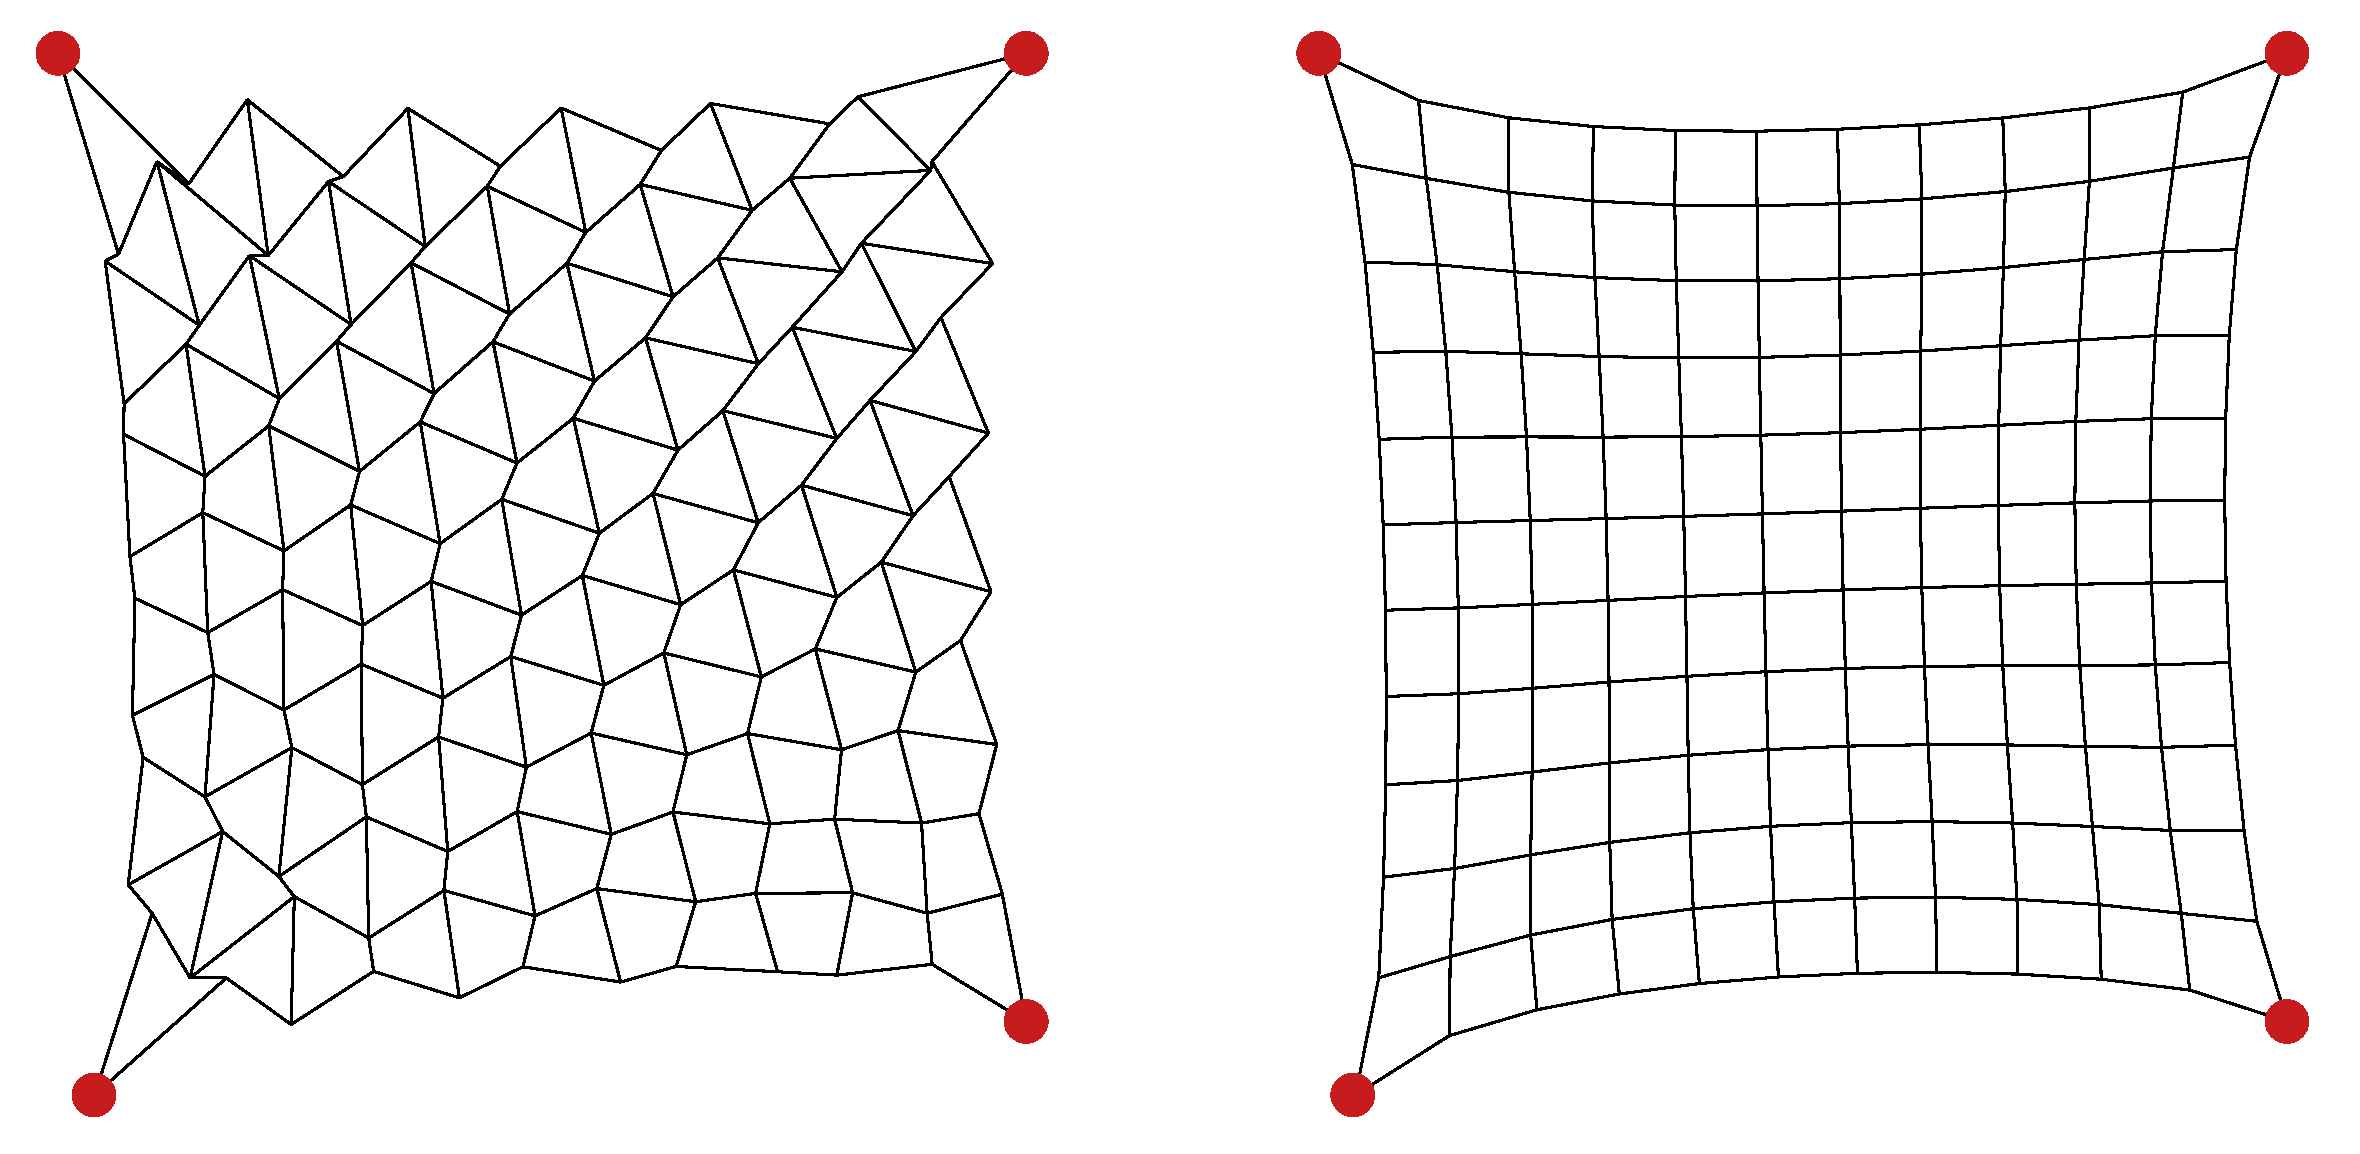
\includegraphics[width=.6\columnwidth]{elasticity/figures/discretization}}
\caption[A 2D comparison of quadrature rules]{A 2D elastic patch is stretched by pinning the four corners to target locations. Left: The unmodified one-point quadrature method is riddled by hourglassing
  instabilities. Right: Our method.}
\vspace{-10pt}
\label{fig_instability}
\end{figure}


\begin{figure}[th]
\centering
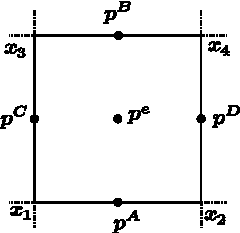
\includegraphics[width=.3\columnwidth]{elasticity/figures/quadrature}
\caption{Our quadrature}
\label{fig_quadrature}
\end{figure}
We remedy this instability by proposing a new integration rule that is
stable yet computationally cheap (requires only one polar decomposition per cell). As an initial observation, we have experimentally verified that the term $\mu\|\mathbf{F}-\mathbf{R}\|_F^2$ in equation (\ref{eqn_energy_F}) is
the one which primarily determines stability; we observed that if a stable technique (e.g.\ 8-point Gauss quadrature) is used to integrate this term, the entire scheme will remain
stable, even if the naive 1-point quadrature is used for the term  $\frac{\lambda}{2}\tr^2(\mathbf{R}^T\mathbf{F}-\mathbf{I})$. Thus, we will initially present our approach in the context
of the simpler energy \newtext{density }$\Psi=\mu\|\mathbf{F}-\mathbf{R}\|_F^2$, and address the 2D case first (\oldtext{e.g.}\newtext{i.e.,}\ on a square lattice). 



\newtext{The use of staggered grids to avoid instability from non-physical modes when using central differencing can be seen in many Eulerian fluid dynamics methods.  }\cite{Harlow:1965:MAC}\newtext{ introduced the staggered MAC grid for velocities and pressure, and }\cite{gerritsma:1996:viscoelastic,Goktekin:2004:viscoelastic}\newtext{ extended this to viscoelastic fluids by staggering the second order stress or strain tensors. Similarly,}  \oldtext{in addition to the cell center $\vec{p}^e$} we introduce four
additional quadrature points $\vec{p}^q,\ q\in\{A,B,C,D\}$, located on edge centers of the quadrilateral lattice as seen in figure (\ref{fig_quadrature}). We write \oldtext{the energy }\newtext{$\Psi$ }as
\begin{equation}
\Psi=\mu\sum_{i,j}
  (F_{ij}-R_{ij})^2.
\label{eqn_energy_only_mu}
\end{equation}
Our approach will essentially follow a different quadrature rule for every term $(F_{ij}-R_{ij})^2$ in this expression. In particular, instead of using the single quadrature point
$\vec{p}^e$ at the cell center, we will use those locations within the cell (possibly more than one) where $F_{ij}$ is ``naturally'' defined, as a central difference of just two degrees
of freedom. In this way, we avoid the averaging and risk of cancellation associated with expressing all derivatives exclusively at the cell center. From figure \ref{fig_quadrature} we
observe that the $x$-derivatives $F_{11}$ and $F_{21}$ are naturally defined at the centers $\vec{p}^A,\vec{p}^B$ of $x$-oriented edges, while the $y$-derivatives $F_{12}$ and $F_{22}$
are naturally located at points $\vec{p}^C$ and $\vec{p}^D$. We also evaluate the cell-centered deformation gradient $\mathbf{F}^e$ once more, following exactly equation
(\ref{eqn_discrete_gradient}) as before. We compute matrix $\mathbf{R}^e$ from the polar decomposition of $\mathbf{F}^e$, and use the information from this matrix wherever $R_{ij}$ is needed 
in equation (\ref{eqn_energy_only_mu}). Finally, our proposed quadrature method takes the form:
\begin{equation}
\!E_e=\frac{\mu h^2}{2}\sum_{i=1}^2\left[\sum_{q\in\{A,B\}}\!\!\!\!\left(F_{i1}^q\!-\!R_{i1}^e\right)^2+\!\!\!\!\sum_{q\in\{C,D\}}\!\!\!\!\left(F_{i2}^q\!-\!R_{i2}^e\right)^2\right].
\label{eqn_quadrature}
\end{equation}
We have that $F_{i1}^e\!=\!\frac{1}{2}\sum_{q\in\{A,B\}}F_{i1}^q$ and $F_{i2}^e\!=\!\frac{1}{2}\sum_{q\in\{C,D\}}F_{i2}^q$ since the entries of $\mathbf{F}^e$ were defined as averaged
central differences. Using these identities, equation (\ref{eqn_quadrature}) becomes $E_e=E_1+E_2$, with
\begin{equation}
E_1=\frac{\mu h^2}{2}\sum_{i=1}^2\left((F_{i1}^A)^2\!+\!(F_{i1}^B)^2\!+\!(F_{i2}^C)^2\!+\!(F_{i2}^D)^2\right),\ \ \mbox{and}
\label{eqn_quadrature_poisson}
\end{equation}
\begin{equation}
E_2=\mu h^2\left[-2\tr\left(\mathbf{R}^{eT}\mathbf{F}^e\right)+\|\mathbf{I}\|_F^2\right]
\label{eqn_quadrature_aux}
\end{equation}
The energy discretization suggested by equations (\ref{eqn_quadrature_poisson}) and (\ref{eqn_quadrature_aux}) is stable, as seen by our results and the convergent multigrid schemes
we have constructed on its basis. In order to better explain the
mechanics of this approach, we manipulate the $\mu$-component of the
energy density as follows:
$$
\Psi=\mu\|\mathbf{F}-\mathbf{R}\|_F^2=\mu\left(\|\mathbf{F}\|_F^2-2\tr\left(\mathbf{R}^T\mathbf{F}\right)+\|\mathbf{I}\|_F^2\right).
$$
Equation (\ref{eqn_quadrature_poisson}) suggests a quadrature rule for the term $\mu\|\mathbf{F}\|_F^2$. The integral $\frac{1}{2}\int\|\mathbf{F}\|_F^2$ is the weak form of the
component-wise Laplace operator; thus equation (\ref{eqn_quadrature_poisson}) generates an energy discretization for the Laplace operator $2\mu\Delta$. Equation
(\ref{eqn_quadrature_aux}) is nothing but a one-point quadrature, but on the term $-2\mu\tr\left(\mathbf{R}^T\mathbf{F}\right)+\mu\|\mathbf{I}\|_F^2$. In fact, at this point we can
re-introduce the omitted $\lambda$-term of the energy, and write $\Psi$ as:
\begin{equation}
\Psi=\underbrace{\mu\|\mathbf{F}\|_F^2}_{\Psi_\Delta}
\underbrace{-2\mu\tr\left(\mathbf{R}^T\mathbf{F}\right)+\mu\|\mathbf{I}\|_F^2+\frac{\lambda}{2}\tr^2(\mathbf{R}^T\mathbf{F}-\mathbf{I})}_{\Psi_{\mbox{\small aux}}}
\label{eqn_psi_poisson_and_aux}
\end{equation}
We implement this discretization, by separating energy, forces, and force differentials into two components: (a) a term stemming from the Laplace energy $\Psi_\Delta$, and (b) an
auxiliary term originating from $\Psi_{\mbox{\small aux}}$, which is integrated with the simple one-point quadrature as in section \ref{sec:elasticity}. Note that the forces arising from
the Laplace term are purely linear, and the stiffness matrix resulting from the same term is constant (and equal to a Laplace matrix), leading to a minimal implementation overhead, over
the standard cost of one-point quadrature for the auxiliary term. 



\section{Indefiniteness correction}
\label{sec:indefiniteness}
Symmetry of the stiffness matrix $\mathbf{K}$ allows the use of certain Krylov
methods, but positive definiteness is required for conjugate gradients. While
$\mathbf{K}$ will be positive definite close to equilibrium (it is the energy
Hessian), in practice Newton-Raphson may generate intermediate
indefinite states. Like \cite{teran:2005:quasistatics}, we will modify
$\mathbf{K}$ to guarantee definiteness while retaining the same nonlinear
solution, a valid equilibrium configuration (though maybe via different iterates).
% \RT{Is this true ? The Newton scheme  will still converge, but will it converge to the same solution ?}
%This
%modified Newton scheme does not change the computed nonlinear solution; the
%algorithm converges to a perfectly valid equilibrium configuration, but while
%iterating through a different sequence of estimates than the original
%Newton-Raphson method.


%in order to use the most efficient variants such as
%conjugate gradients we additionaly require $\mathbf{K}$ to be positive definite. Since  is also the energy Hessian, it will be positive definite in the immediate vicinity of an
%equilibrium configuration. In practice however, for skinning simulations where large skeletal motions between frames are common, the Newton-Raphson procedure will very frequently
%generate indefinite systems before a converged solution is reached. In the spirit of \cite{teran:2005:quasistatics} we will enable the robust use of CG in this context, by modifying
%the stiffness matrix $\mathbf{K}$ so that its definiteness is guaranteed. 

Similar to \cite{teran:2005:quasistatics} we will conservatively enforce the definiteness of $\mathbf{K}$ by projecting each elemental stiffness matrix to its positive semi-definite
counterpart, i.e.\ a matrix with the same eigenvectors, but with negative eigenvalues clamped to zero. Naturally, we want to avoid an explicit eigenanalysis of the $24\times 24$
elemental stiffness $\mathbf{K}^e$, and even avoid forming it at altogether. We describe a procedure to perform this semi-definite projection in an inexpensive, matrix-free fashion. We
will initially describe the definiteness projection for the simple one-point quadrature rule, defined in section \ref{sec:elasticity}. This will be a stepping stone in designing a
definiteness fix for our stabilized quadrature rule, described in
section \ref{sec:stabilization}. 

The elemental stiffness matrix is positive semi-definite if and only if
$0\leq\delta\vec{x}^T\mathbf{K}^e\delta\vec{x}=-\delta\vec{x}^T\delta\vec{f}$, where $\delta\vec{x}$, $\delta\vec{f}$ are the stacked nodal position and force differentials for
$\Omega_e$. Taking differentials on both sides of equation (\ref{eqn_nodal_forces}) we get: 
$$
\delta f_i^{(j)}
=-V_e\sum_k\delta P_{jk}G_{ki}^e
=-V_e\sum_{k,l,m}T_{jklm}\delta F^e_{lm}G_{ki}^e
$$
where $\mathcal{T}=[T_{ijkl}]$ is the fourth order tensor defined as the stress derivative $\mathcal{T}:=\partial\mathbf{P}/\partial\mathbf{F}$, or $T_{ijkl}=\partial P_{ij}/\partial
F_{kl}$. We then write:
\begin{align}
-\delta\vec{x}^T\delta\vec{f}&=-\sum_{i,j}\delta f_i^{(j)}\delta x_i^{(j)}\nonumber\\
&=V_e\!\!\sum_{j,k,l,m}\!\!T_{jklm}\delta F^e_{lm}\sum_iG_{ki}^e\delta
x_i^{(j)}\nonumber\\
&=V_e\!\!\sum_{j,k,l,m}\!\!T_{jklm}\delta F^e_{lm}\delta
F^e_{jk}\nonumber\\
&=V_e\delta\mathbf{F}:\mathcal{T}:\delta\mathbf{F}\label{eqn:K_relation_to_T}
\end{align}
Thus, $\mathbf{K}^e$ will be positive semi-definite, if and only if the fourth order tensor $\partial\mathbf{P}/\partial\mathbf{F}$ is positive definite as well (in the sense that
$\delta\mathbf{F}:\mathcal{T}:\delta\mathbf{F}\geq 0$, for all
$\delta\mathbf{F}$). 

At this point, consider a different 4th order tensor $\hat{\mathcal{T}}$ defined by
$\delta\mathbf{P}=\mathcal{T}:\delta\mathbf{F}=\mathbf{R}[\hat{\mathcal{T}}:(\mathbf{R}^T\delta\mathbf{F})]$. Intuitively, if we define the \emph{unrotated} differentials
$\delta\hat{\mathbf{P}}=\mathbf{R}^T\delta\mathbf{P}$, and $\delta\hat{\mathbf{F}}=\mathbf{R}^T\delta\mathbf{F}$, then $\hat{\mathcal{T}}$ is the tensor that maps
$\delta\hat{\mathbf{P}}=\hat{\mathcal{T}}:\delta\hat{\mathbf{F}}$. Tensors $\mathcal{T}$ and $\hat{\mathcal{T}}$ are a similarity transform of one another; consequently they share the
same eigenvalues, and performing the indefiniteness fix on one will guarantee the definiteness of the other. Using this definition and equations (\ref{eqn_stress_differential}) and
(\ref{eqn_rotation_differential}), $\delta\hat{\mathbf{P}}$ reduces to:
\begin{equation}
\delta\hat{\mathbf{P}}=\hat{\mathcal{T}}:\delta\hat{\mathbf{F}}=
2\mu\delta\hat{\mathbf{F}}\!+\!\lambda\tr(\delta\hat{\mathbf{F}})\mathbf{I}\!+\!\left\{\lambda\tr(\mathbf{S}\!-\!\mathbf{I})\!-\!2\mu\right\}\mathcal{S}\!:\!\delta\hat{\mathbf{F}}
\label{eqn_rotated_dp}
\end{equation}
where $\mathcal{S}=\mathcal{E}:\left\{\tr(\mathbf{S})\mathbf{I}-\mathbf{S}\right\}^{-1}:\mathcal{E}^T$. Consider the decomposition of
$\delta\hat{\mathbf{F}}\!=\!\delta\hat{\mathbf{F}}_{\mbox{\small sym}}\!+\!\delta\hat{\mathbf{F}}_{\mbox{\small skew}}$ into symmetric 
$\delta\hat{\mathbf{F}}_{\mbox{\small sym}}\!=\!(\delta\hat{\mathbf{F}}\!+\!\delta\hat{\mathbf{F}}^T)/2$ and skew symmetric
$\delta\hat{\mathbf{F}}_{\mbox{\small skew}}\!=\!(\delta\hat{\mathbf{F}}\!-\!\delta\hat{\mathbf{F}}^T)/2$ parts; also consider a similar decomposition of 
$\delta\hat{\mathbf{P}}\!=\!\delta\hat{\mathbf{P}}_{\mbox{\small sym}}\!+\!\delta\hat{\mathbf{P}}_{\mbox{\small skew}}$. By collecting symmetric and skew symmetric terms from equation
(\ref{eqn_rotated_dp}) we have:

\begin{equation}
\delta\hat{\mathbf{P}}_{\mbox{\small sym}}=2\mu\delta\hat{\mathbf{F}}_{\mbox{\small sym}}\!+\!\lambda\tr(\delta\hat{\mathbf{F}}_{\mbox{\small sym}})\mathbf{I}=\mathcal{T}_{\mbox{\small sym}}:\delta\hat{\mathbf{F}}_{\mbox{\small sym}}
\label{eqn_dp_sym}
\end{equation}
\begin{equation}
\hspace*{-.2in}\delta\hat{\mathbf{P}}_{\mbox{\small skew}}
\!=\!2\mu\delta\hat{\mathbf{F}}_{\mbox{\small skew}}\!+\!\left\{\lambda\tr(\mathbf{S}\mbox{-}\mathbf{I})\mbox{-}2\mu\right\}\mathcal{S}\!:\!\delta\hat{\mathbf{F}}_{\mbox{\small skew}}
\!=\!\mathcal{T}_{\mbox{\small skew}}\!:\!\delta\hat{\mathbf{F}}_{\mbox{\small skew}}
\label{eqn_dp_skew}
\end{equation}

In essence, $\hat{\mathcal{T}}=\mathcal{T}_{\mbox{\small sym}}+\mathcal{T}_{\mbox{\small skew}}$ has a fully decoupled action on the two subspaces of symmetric, and skew symmetric
matrices. Since the symmetric and skew subspaces are orthogonal, $\hat{\mathcal{T}}$ will be semi-definite, if and only if its skew and symmetric parts are semi-definite too. The
tensor $\mathcal{T}_{\mbox{\small sym}}=2\mu\mathcal{I}_{\mbox{\small sym}}+\lambda\mathbf{I}\otimes\mathbf{I}$ ($\mathcal{I}_{\mbox{\small sym}}$ is the operator that projects a
matrix onto its symmetric part) is always positive semi-definite; thus no modification is necessary. If $\mathcal{I}_{\mbox{\small skew}}$ is the operator that projects a matrix onto
its skew symmetric part, we can verify that $2\mathcal{I}_{\mbox{\small skew}}=\mathcal{E}:\mathbf{I}:\mathcal{E}^T$. Thus, $\mathcal{T}_{\mbox{\small skew}}$ is written as:
$$
\mathcal{T}_{\mbox{\small skew}}=\mu\mathcal{E}:\mathbf{I}:\mathcal{E}^T+\left\{\lambda\tr(\mathbf{S}\!-\!\mathbf{I})\!-\!2\mu\right\}\left[\mathcal{E}\!:\!\left\{\tr(\mathbf{S})\mathbf{I}\!-\!\mathbf{S}\right\}^{-1}\!:\!\mathcal{E}^T\right]
$$
$$
=\mathcal{E}\!:\!\mathbf{L}\!:\!\mathcal{E}^T,\ \mbox{where}\ \mathbf{L}=\mu\mathbf{I}+\left\{\lambda\tr(\mathbf{S}\!-\!\mathbf{I})\!-\!2\mu\right\}\left\{\tr(\mathbf{S})\mathbf{I}\!-\!\mathbf{S}\right\}^{-1}
$$

$\mathcal{E}$ is also an orthogonal (although not orthonormal) tensor, thus the definiteness of $\mathcal{T}_{\mbox{\small skew}}$ is equivalent with the definiteness of the $3\times 3$ 
symmetric matrix $\mathbf{L}$, which can be easily projected to its positive definite part. In fact, if the method we used to compute the polar decomposition were to first compute the
entire SVD $\mathbf{F}=\mathbf{U}\mathbf{\Sigma}\mathbf{V}^T$ of the deformation gradient, then we have $\mathbf{L}=\mathbf{V}\mathbf{L}_D\mathbf{V}^T$ where
$$
\mathbf{L}_D=\mu\mathbf{I}+\left\{\lambda\tr(\mathbf{\Sigma}\!-\!\mathbf{I})\!-\!2\mu\right\}\left\{\tr(\mathbf{\Sigma})\mathbf{I}\!-\!\mathbf{\Sigma}\right\}^{-1}
$$
is a diagonal matrix, whose diagonal entries simply need to be clamped to zero, to ensure definiteness for $\mathbf{L}$, for $\mathcal{T}_{\mbox{\small skew}}$ and ultimately for the entire
element stiffness matrix. 

In practical implementation, the matrix $\mathbf{L}$, projected to its semi-definite component, is precomputed and stored at the same time when the Polar Decomposition
of each element is performed. Then, the definitions of this section are followed to successively construct 
$\delta\hat{\mathbf{P}}_{\mbox{\small sym}}$ and \ $\delta\hat{\mathbf{P}}_{\mbox{\small skew}}$, using equations (\ref{eqn_dp_sym}),(\ref{eqn_dp_skew}), and ultimately
$\delta\mathbf{P}=\mathbf{R}\delta\hat{\mathbf{P}}$. 

So far, we have discussed how to correct the indefiniteness of the stiffness matrix arising from the (unstable) one-point quadrature technique. In light of the energy decomposition reflected
in equation (\ref{eqn_psi_poisson_and_aux}) the difference in the discrete energy between the stable and unstable approaches, is the discrete quadrature that will be followed to
integrate the part $\Psi_\Delta$. Our stable technique employs equation (\ref{eqn_quadrature_poisson}) for this task, while the original unstable technique uses one-point
quadrature. In two spatial dimensions, if we denote by $E_\Delta^S$ and $E_\Delta^U$ the discrete integral associated with the Laplace term in the stable, and unstable variants
respectively, we then have:
\begin{eqnarray*}
E_\Delta^U&=&\mu h^2\sum_{i=1}^2\left((F_{i1}^e)^2+(F_{i2}^e)^2\right)\\
&=&\mu h^2\sum_{i=1}^2\left((\frac{F_{i1}^A+F_{i1}^B}{2})^2+(\frac{F_{i2}^C+F_{i2}^D}{2})^2\right)
\end{eqnarray*}
\begin{equation}\label{eqn:stable_definite}
E_\Delta^U-E_\Delta^S\stackrel{\mbox{\small(\ref{eqn_quadrature_poisson})}}{=}\mu h^2\sum_{i=1}^2\left((\frac{F_{i1}^A-F_{i1}^B}{2})^2+(\frac{F_{i2}^C-F_{i2}^D}{2})^2\right)\geq 0
\end{equation}
Thus, we can interpret our stable discretization as adding the unconditionally convex term $E_\Delta^U-E_\Delta^S$ to the unstable energy discretization of the single-point
approach. 

The indefiniteness fix described in the context of the unstable method can also be interpreted as augmenting the real stiffness matrix with a supplemental term
$\mathbf{K}\gets\mathbf{K}+\mathbf{K}_{\mbox{\small supp}}$ that guarantees the definiteness of the resulting matrix.  Equation~(\ref{eqn:stable_definite})  indicates that if the same
``definiteness-boosting'' matrix $\mathbf{K}_{\mbox{\small supp}}$ is added to the stable discretization, definiteness will be guaranteed. 

Algorithm \ref{alg_indefiniteness_fix}
summarizes the entire procedure that implements the ``auxiliary'' stress differential corresponding to the $\Psi_{\mbox{\small aux}}$ energy component. The differential of the
additional force due to the Laplace term $\Psi_\Delta$ are computed as described in section \ref{sec:stabilization}.
\begin{algorithm}[h]
\caption{Computation of the stress differential corresponding to the auxiliary energy term $\Psi_{\mbox{\small aux}}$. Fixed to guarantee definiteness.}
\label{alg_indefiniteness_fix}
\begin{algorithmic}[1]
\Function{Compute\_L}{$\mathbf{\Sigma},\mathbf{V},\mu,\lambda,\mathbf{L}$}
\State $\mathbf{L}_D\gets\left\{\lambda\tr(\mathbf{\Sigma}\!-\!\mathbf{I})\!-\!2\mu\right\}\left\{\tr(\mathbf{\Sigma})\mathbf{I}\!-\!\mathbf{\Sigma}\right\}^{-1}$
\State Clamp diagonal elements of $\mathbf{L}_D$ to a minimum value
of $(-\mu)$\Comment{Term $\Psi_\Delta$ will boost this eigenvalue by $\mu$}
\State $\mathbf{L}\gets\mathbf{V}\mathbf{L}_D\mathbf{V}^T$
\EndFunction
\Function{dPauxDefiniteFix}{$\delta\mathbf{F},\mathbf{R},\mathbf{L}$}\Comment{Returns $\delta \mathbf{P}_{\mbox{\small aux}}$}
\State $\delta\hat{\mathbf{F}}_{\mbox{\small sym}}\gets\Call{SymmetricPart}{\mathbf{R}^T\delta\mathbf{F}}$
\State $\delta\hat{\mathbf{F}}_{\mbox{\small skew}}\gets\Call{SkewSymmetricPart}{\mathbf{R}^T\delta\mathbf{F}}$
\State $\delta\hat{\mathbf{P}}_{\mbox{\small sym}}\gets\lambda\tr(\delta\hat{\mathbf{F}}_{\mbox{\small sym}})\mathbf{I}$
\State $\delta\hat{\mathbf{P}}_{\mbox{\small skew}}\gets\mathcal{E}\!:\!\left\{\mathbf{L}(\mathcal{E}^T\!:\!\delta\hat{\mathbf{P}}_{\mbox{\small skew}})\right\}$
\State $\delta\mathbf{P}_{\mbox{\small aux}}\gets\mathbf{R}\left(\delta\hat{\mathbf{P}}_{\mbox{\small sym}}+\delta\hat{\mathbf{P}}_{\mbox{\small skew}}\right)$
\State \Return $\delta\mathbf{P}_{\mbox{\small aux}}$
\EndFunction
\end{algorithmic}
\end{algorithm}



\section{Dynamics}
Our method extends trivially to dynamic simulations that include inertial effects. However, it is important to note that the indefiniteness encountered in quasistatic time stepping also arises in implicit time stepping for dynamics. Fortunately, the definiteness fix outlined above can be used in this setting as well. Here we will outline why this indefiniteness is increasingly likely to occur when performing interactive high-resolution simulation. In this case, we typically desire a fixed temporal resolution of $\Delta{t}\approx\frac{1}{30}$ (to take as few timesteps as possible). 

Using the common backward Euler time stepping scheme for illustration, and assuming that the resulting non-linear equations are solved with Newton-Raphson's method, the following update equation must be solved for the increment $\delta\vec{{x}}$ in the $k^\textrm{th}$ iteration:
\begin{align}
\mathbf{K}^{BE}(\mathbf{x}^{n+1}_k)\delta\mathbf{x} &= \mathbf{f}(\mathbf{x}^{n+1}_k) + \mathbf{g}+\mathbf{M}\left(\left(\mathbf{x}^n-\mathbf{x}^{n+1}_k\right)/\Delta t^2 + \mathbf{v}^n/\Delta t\right)\nonumber\\
\mathbf{x}^{n+1}_{k+1}&=\mathbf{x}^{n+1}_k+\delta\mathbf{x}\label{eqn:backward_euler}
\end{align}
% To demonstrate this fact, let us examine the comparatively simple case of backward Euler time stepping. Here, our discrete system of equations is:
% $$
% \frac{\vec{x}^{n+1}-\vec{x}^{n}}{\Delta{t}} = \vec{v}^{n+1}\ \ \mbox{and}\ \ 
% \mathbf{M}\left(\frac{\vec{v}^{n+1}-\vec{v}^{n}}{\Delta{t}}\right) = \vec{f}(\vec{x}^{n+1})
% $$
% where $\mathbf{M}$ is the mass matrix associated with the material of interest. 
% %
% % For example, in a finite element based discretization one would use $M_{ij}=\int_{\Omega_0}{\rho(\mathbf{X})}{N_i}{N_j}d\mathbf{X}$ where $N_i$ and $N_j$ are the interpolating functions associated with each degree of freedom and $\rho$ is the mass density of the material. However, in graphics it is common to use a diagonal approximation (or mass lumping approximation) to this matrix obtained by summing each row: $M^\textrm{d}_{ii}=\sum_jM_{ij}$. This is equivalent to assigning each node an equal portion of volume of each of its incident elements and then determining the mass of the node as density times this volume. For example, in a tetrahedron based approximation each node would be given one fourth of the volume of each of its incident tetrahedra. 
% %
% We can solve this non-linear system by first eliminating $\vec{v}^{n+1}$ to get
% $$
% \mathbf{M}\left(\vec{x}^{n+1}-\vec{x}^{n}\right) = \Delta{t}\mathbf{M}\vec{v}^n + \Delta{t}^2\vec{f}(\vec{x}^{n+1})
% %\mathbf{M}\left(\frac{\frac{\vec{x}^{n+1}-\vec{x}^{n}}{\Delta{t}}-\vec{v}^{n}}{\Delta{t}}\right)=\vec{f}(\vec{x}^{n+1})
% $$
%% and then performing Newton iteration for $\vec{x}^{n+1}$. At the $k^\textrm{th}$ Newton iteration, we update an approximation to $\vec{x}^{n+1}$ given by $\vec{x}^{n+1}_{k+1}= \vec{x}^{n+1}_{k}+ \vec{\delta{x}}$ by solving the system
%$$
%\mathbf{K}^\textrm{BE}(\vec{x}^{n+1}_{k}) \delta\vec{{x}}=\Delta{t}\mathbf{M} \vec{v}^n+\Delta{t}^2 \vec{f}(\vec{x}^{n+1}_{k})
%$$
Here $\mathbf{K}^{BE}(\mathbf{x}^{n+1}_k) = \mathbf{M}/\Delta{t}^2+\mathbf{K}(\vec{x}^{n+1}_{k})$, and $\mathbf{M}$ is the mass matrix. 

The indefiniteness of $\mathbf{K}(\vec{x}^{n+1}_{k})$ can thus be seen to potentially cause indefiniteness of the backward Euler system matrix $\mathbf{K}^\textrm{BE}(\vec{x}^{n+1}_{k})$. Specifically, there are three factors that will conspire to yield indefiniteness in the  backward Euler system matrix: time step size ($\Delta{t}$), nodal mass ($M_{ii}$) and relative magnitude of elasticity parameters ($\mu$,$\lambda$). It may be tempting to adjust these parameters to provide a definite backward Euler system matrix. For example larger nodal mass, smaller $\Delta{t}$ and smaller $\mu,\lambda$ have a better chance of yielding a definite matrix. However, altering the nodal mass or elasticity coefficients would be equivalent to altering the behavior of the material inherent in the governing equations and should therefore be considered off limits. Secondly, when interactivity is desired the time step cannot be decreased arbitrarily. Furthermore, it is important to note that the nodal mass is proportionate to the volume associated with each node. Therefore, as we increase the discrete spatial resolution of our domain, the nodal mass decreases thereby increasing the likelihood of encountering an indefinite backward Euler system matrix as it would behave more and more like the indefinite $\mathbf{K}(\vec{x}^{n+1}_{k})$. Therefore, we see that when maximum performance and high resolution are desired, indefiniteness in the backward Euler system matrix is a distinct possibility. Fortunately, the definiteness fix outline above for $\mathbf{K}(\vec{x}^{n+1}_{k})$ suffices to guarantee definiteness of the backward Euler system matrix.



\section{Constraints and collisions}
\label{sec:constraints}


\begin{figure}
\begin{center}
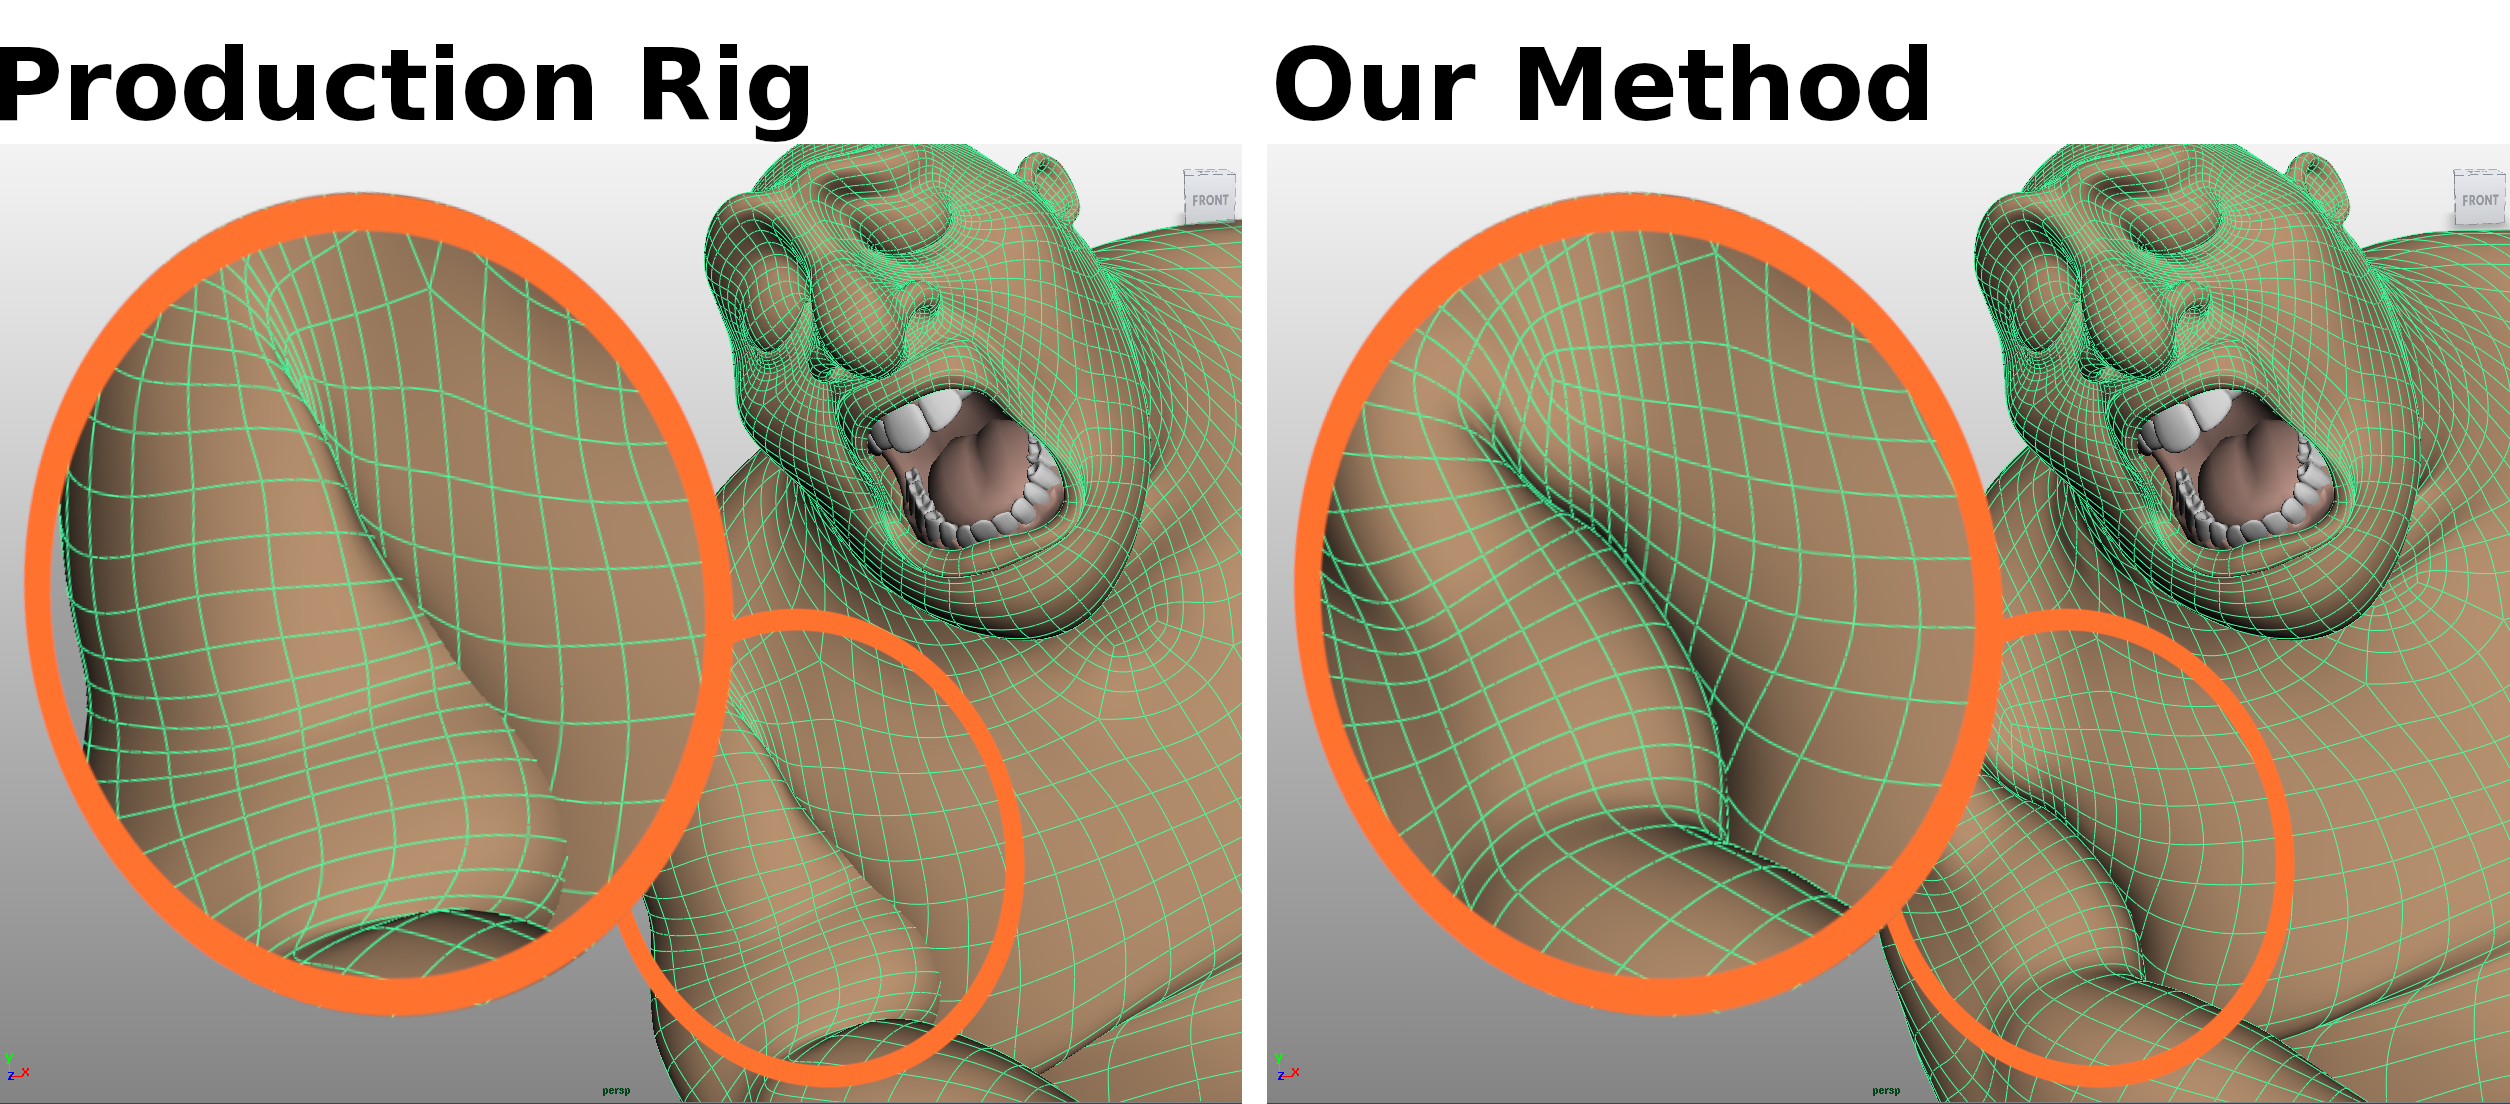
\includegraphics[width=\linewidth]{elasticity/figures/collision-figure}
\end{center}
\caption[Collisions improve deformation quality.]{Collisions and especially self-collisions drastically improve the
  quality of deformation when coupled with elasticity. On the left is a
  production rig that qualitatively exhibits the right look but does not resolve
  collisions. On the right is our method which resolves self-collisions
  producing a much more natural look. Images \copyright Disney. All rights reserved.}
\label{fig:collisions}
\end{figure}

As previously discussed, the ability to handle elaborate collision is an essential benefit of simulation in production. We use point constraints to enforce both soft constraints, such as bone attachments, and to handle object and self collisions. Specifically, we embed proxy points ($\mathbf{x}_p$) in the simulation lattices and distribute their associated forces trilinearly to the vertices of the hexahedral cells that contain them. \cite{sifakis:2007:hybridsolids} show the effectiveness of this basic approach.

\paragraph{Soft constraints }
Springs attached to embedded proxy points are used to enforce soft constraints such as bone bindings. The forces from these springs are derived from the standard quadratic energy density
$\Psi(\mathbf{x}) = k/2\|\mathbf{x}-\mathbf{x}_p\|^2$.

\paragraph{Collision detection }
The collision response is determined by a number of collision proxies approximately covering the embedded collision surface. We utilize a penalty based response dependent on the penetration depth and unit outward normal at each proxy point. For rigid objects, we simply query a level set representation of the object at each proxy point. However, for self-collision, the rapidly changing shape of the elastic objects precludes accurate reconstruction of a signed distance function at each time step.

\paragraph{Self-collision penetration depth evaluation }
For each proxy collision point, we first determine which deformed hexahedra contain it in the current configuration. This is done rapidly by querying an axis aligned bounding box hierarchy whose leaves surround each deformed hexahedron in the current configuration. To prevent false positives, we do not look in the 27 hexahedra in the one ring of the proxy point in material coordinates. Each hexahedron deemed near a given proxy point is then tetrahedralized to barycentrically determine the proxy point's material location. For each material point, we query a level set stored in the undeformed configuration: $\phi_0$.  If there are multiple negative $\phi_0$ values, we use the location with $\phi_0$ closest to zero to compute the closest point on the undeformed surface. We then look up the deformed position of the closest surface point ($\mathbf{x}_s$)  to estimate the penetration depth as $\left|\mathbf{x}_s-\mathbf{x}_p\right|$ and outward unit normal as $\mathbf{n}=\left(\mathbf{x}_s-\mathbf{x}_p\right)/\left|\mathbf{x}_s-\mathbf{x}_p\right|$.

\paragraph{Collision response }
For both self-collision and solid object collision scenarios, we instantiate a zero rest-length spring from the proxy point to the closest point on the surface. The Young's modulus of this spring is allowed to be anisotropic in the direction of the unit collision normal. Specifically, the spring force arises from the energy density
$\Psi(\mathbf{x}_p,\mathbf{x}_s)=k(\mathbf{x}_p-\mathbf{x}_s)^T\mathbf{M}(\mathbf{x}_p-\mathbf{x}_s)/2$
where  $\mathbf{M}=\left(1-\alpha\right)\mathbf{n}\mathbf{n}^T+\alpha\mathbf{I}$, with $\alpha\in[0,1]$.  $\alpha=1$ corresponds with a traditional isotropic spring; $\alpha=0$ results in a standard point repulsion.  This anisotropic conception of the stiffness allows for sliding in the plane orthogonal to the penetration direction. In practice we found $\alpha\in[.1,.5]$ worked best for self collisions and $\alpha = 0$ was sufficient for object collisions.


\section{Multigrid}
\label{sec:multigrid}
To ensure that our method scales to high resolutions, we solve the equations of elasticity using a multigrid technique. In fact, we explored two possible approaches: the first option is to construct a multigrid cycle purely as a solver for
the linear system (\ref{eqn_newton_step}) generated in every Newton-Raphson step. The other possibility is to implement a fully nonlinear multigrid cycle, based on the Full
Approximation Scheme (FAS) which would replace and accelerate the entire sequence of Newton iterations. This section details several design subtleties, and algorithmic modifications
that were necessary to efficiently implement these two multigrid schemes. 

\paragraph{Domain description} Our discretization is based on a voxelized representation of the elastic body. At any given resolution, a cubic background lattice is defined and
its cells are labeled either \emph{internal} or \emph{external} depending on any material overlap with the embedded deforming body. Internal cells can optionally be labeled as
\emph{constrained} (or Dirichlet) if the trajectories of their nodes will be specified as hard kinematic constraints. The Lam\'{e} coefficients $\mu$ and $\lambda$ can be specified for
each individual cell, allowing for inhomogeneous models. The coarser domains of a multigrid hierarchy are generated by a simple binary coarsening strategy. Similar to
\cite{Zhu:2010:EMM} a label of constrained, internal or external is assigned in this order of priority, if fine children with more than one type are present. The Lam\'{e} parameters of
coarse interior cells are computed by summing the $\mu$ or $\lambda$ of any \emph{interior} children, and dividing by eight; thus coarse cells overlapping with the boundary receive
lower material parameters, to account for the partial material coverage of the cell.

\paragraph{Elasticity coarsening} A multigrid method requires us to generate a hierarchy of discretizations. Specifically, if we use multigrid to solve the linear system
(\ref{eqn_newton_step}), different versions of $\mathbf{K}$, denoted by $\mathbf{K}^h,\mathbf{K}^{2h},\mathbf{K}^{4h},\ldots$ need to be computed for every level of the multigrid
hierarchy. We specifically avoid the Galerkin coarsening strategy since it requires forming the stiffness matrices explicitly. The alternative is a 
matrix-free approach which constructs $\mathbf{K}^{2h}$ from a re-discretization of our problem at the coarse grid. We can repeat the same process followed at the fine grid, and
define coarse forces $\vec{f}^{2h}(\vec{x}^{2h})=-\partial\Psi^{2h}/\partial\vec{x}^{2h}$ as well as a coarse stiffness $\mathbf{K}^{2h}=\partial\vec{f}^{2h}/\partial\vec{x}^{2h}$ and
encode these in a matrix-free fashion as before. The challenge however is that the entries in $\mathbf{K}^{2h}$ depend on the current estimate of the solution and, more accurately, on a
\emph{coarse grid} version $\vec{x}^{2h}$ of this estimate. The general methodology is to define yet another restriction operator $\hat{\mathbf{R}}$ (possibly different than the
$\mathbf{R}$ used to restrict residuals) to downsample the solution estimate as $\vec{x}^{2h}=\hat{\mathbf{R}}\vec{x}^h$. However, as a consequence of our geometric domain coarsening
described in the previous paragraph, the discrete domain \emph{grows} in size, as coarse cells with any interior children will now be considered fully interior, even if they include some
exterior cells from the fine grid. Therefore, restricting the approximation $\vec{x}^h$ would require extrapolation of the deformation field. We found such extrapolations to be
quite unstable, especially in the presence of collisions, and sometimes even ill-defined near concave, high curvature boundaries.

Our solution is based on the observation that the entries of $\mathbf{K}$ do not depend directly on the positions $\vec{x}$, but only through the deformation gradient $\mathbf{F}$. Note
that this is also true for our stabilized discretization; the part $\mathbf{K}_\Delta$ of the stiffness matrix due to $\Psi_\Delta$ is a \emph{constant} matrix, not dependent on positions
at all. The auxiliary part $\mathbf{K}_{\mbox{\small aux}}$ due to $\Psi_{\mbox{\small aux}}$ is fully determined by the discrete deformation gradient $\mathbf{F}^e$ at every
cell. Thus, instead of restricting $\vec{x}^h\rightarrow\vec{x}^{2h}$ we instead downsample the deformation gradient as $\mathbf{F}^h\rightarrow\mathbf{F}^{2h}$, which is done with
simple weighted averaging. Once the stiffness matrices have been constructed for all levels, the V-Cycle described in Algorithm \ref{alg_linear_vcycle} is used to solve the linearized
Newton equation. The transfer operators $\mathbf{R}$ and $\mathbf{P}$ are constructed based on trilinear interpolation. Since we do not explicitly construct $\mathbf{K}$, we use a
Jacobi smoother instead of a Gauss-Seidel one, since for the Jacobi procedure all force differentials may be computed in parallel. Note however that the elasticity matrix is not
diagonally dominant, and the Jacobi procedure needs to be damped for stable convergence. We found that the damping coefficient could safely be as high as $0.8$ in the interior of the
object, while values of $0.3-0.4$ were more appropriate near the boundary, near soft constraints, and for higher values of Poisson's ratio.

\begin{algorithm}[h]
\caption{Linear Multigrid V(1,1) Cycle for equation (\ref{eqn_newton_step})}\label{alg_linear_vcycle}
\begin{algorithmic}[1]
\Procedure{LinearVCycle}{}
\State $\vec{b}^h\gets \vec{f}^h(\vec{x}^h)+\vec{g}^h$
\For{$l= 0 \textbf{\ to\ }L$$-$$1$}\Comment{total of $L$$+$$1$ levels}
\State Smooth($\mathbf{K}^{2^lh}$,$\delta\vec{x}^{2^lh}$,$\vec{b}^{2^lh}$)
\State $\vec{r}^{2^lh}\gets\vec{b}^{2^lh}-\mathbf{K}^{2^lh}\delta\vec{x}^{2^lh}$
\State $\vec{b}^{2^{l+1}h}\gets$Restrict($\vec{r}^{2^lh}$),\ $\delta\vec{x}^{2^{l+1}h}\gets 0$
\EndFor
\State Solve $\delta\vec{x}^{2^Lh}\gets (\mathbf{K}^{2^Lh})^{-1}\vec{b}^{2^Lh}$
\For{$l=L$$-$$1 \textbf{\ down to\ } 0$}
\State $\delta\vec{x}^{2^lh}\gets \delta\vec{x}^{2^lh}+$Prolongate($\delta\vec{x}^{2^{l+1}h}$)
\State Smooth($\mathbf{K}^{2^lh}$,$\delta\vec{x}^{2^lh}$,$\vec{b}^{2^lh}$)
\EndFor
\EndProcedure
\end{algorithmic}
\end{algorithm}

\paragraph{Point constraint coarsening} Each soft constraint and active collision proxy is copied to the coarse grids based on its material location.  Its associated stiffness modulus is scaled by a factor of .125 (or .25 in 2D) to accommodate its embedding in a larger element.  Otherwise, the coarsened proxies are then treated in the same manner at every level of the hierarchy.

\paragraph{Nonlinear multigrid} We also implemented a fully nonlinear multigrid
solver, based on the Full Approximation Scheme (FAS) approach. As before, the
challenge is  that the nonlinear force operator requires a coarse grid version of the solution estimate. Once
again, the operator only depends on $\vec{x}$ through the deformation gradient;
unfortunately the deformation gradient does not stay fixed through smoothing and
v-cycles, requiring constant updates.  We consider the restricted value of the
deformation gradient as an ``offset'' (denoted by $\mathbf{F}_{\mbox{\small off}}$) and change
our state variables for the coarser grids from \emph{positions} ($\vec{x}$) to
\emph{corrections} ($u$) from this offset. We compute the updated deformation  as
$\mathbf{F}=\mathbf{F}_{\mbox{\small off}}+\mathbf{G}[\vec{u}]$, where
$\mathbf{G}$ is the cell-centered gradient operator. The nonlinear forces
computed based on this updated gradient are 
$\vec{f}^h(\mathbf{F}_{\mbox{\small off}}^h;\vec{u}^h)$. The FAS procedure is
outlined in Algorithm
\ref{alg_fas_vcycle}. Damped Jacobi is used, albeit with re-linearization steps inserted between every 2-3 Jacobi iterations.

\begin{algorithm}[h]
\caption{FAS V-Cycle  for nonlinear equilibrium equation}\label{alg_fas_vcycle}
\begin{algorithmic}[1]
\Procedure{FASVcycle}{$\vec{f}^h(\mathbf{F}_{\mbox{\small off}}^h;\vec{u}^h)+\vec{g}^h=\vec{0}$}
\State \Call{NonlinearSmooth}{$\vec{f}^h(\mathbf{F}_{\mbox{\small off}}^h;\vec{u}^h)+\vec{g}^h=\vec{0}$}
\State $\mathbf{F}_{\mbox{\small off}}^{2h}\gets\hat{\mathbf{R}}(\mathbf{F}_{\mbox{\small off}}^h+\mathbf{G}^h[\vec{u}^h]),\vec{u}^{2h}\gets\vec{0}$
\State $\vec{g}^{2h}\gets-\vec{f}^{2h}(\mathbf{F}_{\mbox{\small off}}^{2h};\vec{u}^{2h})+\mathbf{R}(\vec{f}^h(\mathbf{F}_{\mbox{\small off}}^h;\vec{u}^h)+\vec{g}^h)$
\State \Call{Solve}{$\vec{f}^{2h}(\mathbf{F}_{\mbox{\small off}}^{2h};\vec{u}^{2h})+\vec{g}^{2h}=\vec{0}$}\Comment{By recursive call}
\State $\vec{u}^{h}\plusequals $Prolongate($\vec{u}^{2h}$)
\State \Call{NonlinearSmooth}{$\vec{f}^h(\mathbf{F}_{\mbox{\small off}}^h;\vec{u}^h)+\vec{g}^h=\vec{0}$}
\EndProcedure
\end{algorithmic}
\end{algorithm}

Our experiments with the fully nonlinear FAS cycle exhibited significant acceleration in certain tasks, but was somewhat more questionable in terms of cost/performance for our typical
use scenario. In particular, when solving for the equilibrium shape following a very sudden skeletal motion (such as fully curling an arm from a full extension, all in a single frame),
the FAS scheme was able to converge in just a few cycles, while the linear multigrid approach would typically necessitate a large number of Newton iterations (even though each linear
system was adequately solved). However, in our typical use, the skeletal motion was relatively incremental, and 1-2 Newton iterations would provide an excellent solution estimate, with
1-2 linear V-cycles as the underlying linear solver. Since the linear cycle is less expensive due to less frequent re-linearization, this approach was overall a better cost/performance
choice for our specific application. Additionally, in the presence of collisions, extreme skeletal motions within a single frame were problematic, since the penalty-based collisions
would easily become tangled in nonphysical configurations. Lastly, we observed that the ability of FAS to make large corrections towards the solution often times had the side effect of
sometimes jumping between different local minima, especially in highly buckled configurations. This behavior can be controlled by augmenting FAS with a linesearch step to prevent it
from tunneling to different minima, but again this was not a priority for our target application.


\section{Optimization}
\label{sec:implementation}
\begin{figure}[tb]
\center{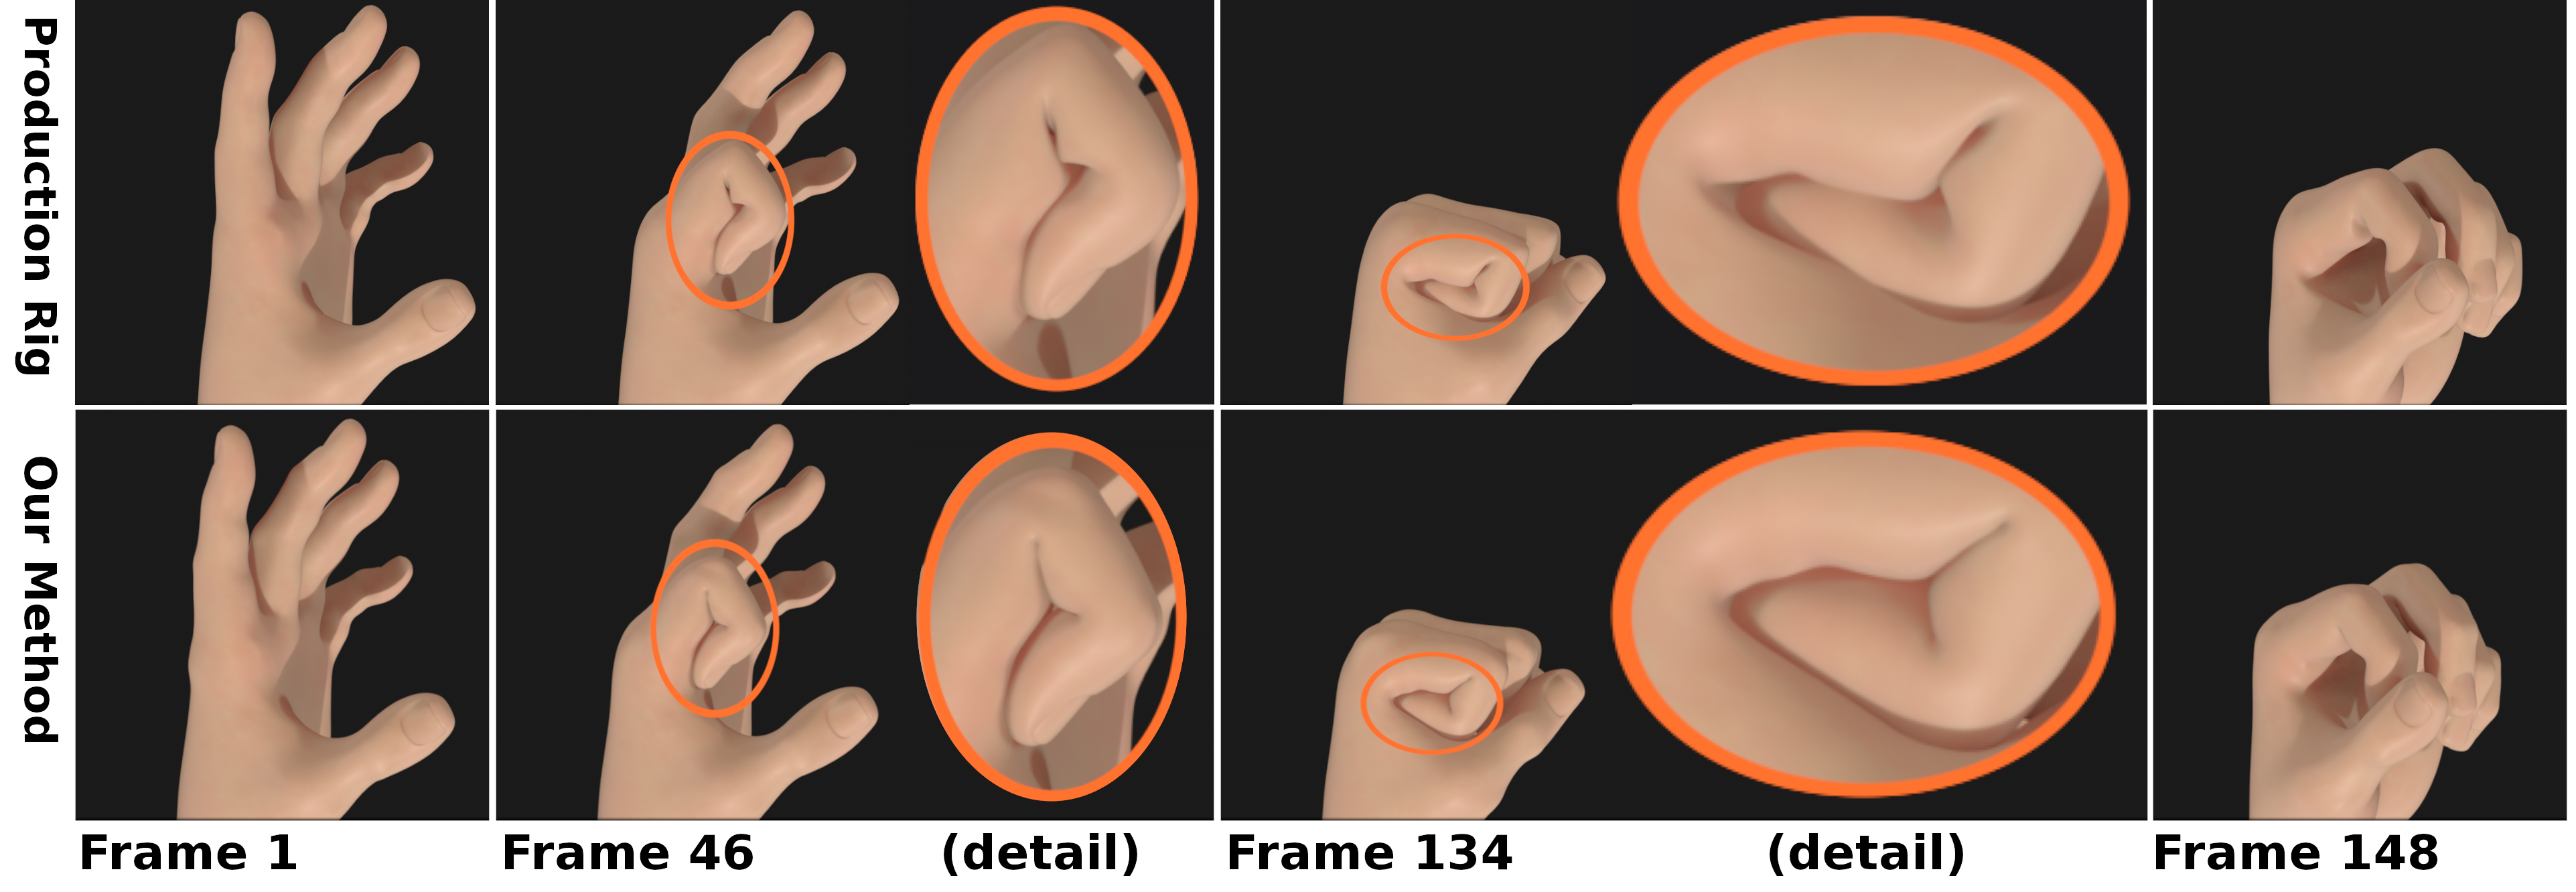
\includegraphics[width=1\linewidth]{elasticity/figures/handfigure}}
\caption[A hand rigged using linear blend skinning and our method.]{Top: A hand rigged using linear blend skinning. Due to the many joints
it is impractical to model all the shapes necessary fix the artifacts using an
example based technique like PSD. To compensate, a significant amount of effort was
spent on creating a nice skin bind for this hand. Bottom: The same hand rigged with our
elasticity based deformer using 117,607 non-empty cells. Note how we get correct creasing and contact
deformation where the finger bends.}
\label{fig:hand}
\end{figure}


\paragraph{Initial guess.} A very significant source of optimization is the choice of initial guess because
we use iterative methods.  To make solutions deterministic and completely frame
independent we considered the use of a base linear blend skin as an initial
guess. However, this can lead to unstable behavior in the presence of large
contact deformations because collision resolution is path dependent. Instead, we therefore use the previous
solution (often the previous frame) as an initial guess. 

\paragraph{CPU.} To improve performance on the CPU we utilized multithreading using a task
queue. We designed our access patterns to be cache friendly by using blocking
techniques.  We also exploited SSE data level parallelism for the SVD
computation. Additionally, we used templatization to optimize stride
multiplication computations in array accesses. Constraint contributions to the
matrix were baked into a structure that minimized indirection.

\paragraph{GPU.} Since GPUs have become popular for parallel numerical algorithms, we did a
na\"{i}ve port of our CPU oriented code to the GPU. Our expertise at optimizing
for the GPU's different bandwidth versus computation tradeoffs was limited, and
we hope to utilize the grid optimization techniques of \cite{Dick:2011:CUDAFEM}
in the future.

We benchmarked our elasticity multigrid solver on a cube model with Dirichlet constraints on two opposite faces without collisions or point constraints. While we were able to attain a
convergent method with as few as 2 Jacobi smoothing sweeps per grid transfer, we were able to achieve the best balance between speed and convergence rate with 5-10 Jacobi relaxation
sweeps.  In all cases, the first V-cycles significantly (by 1-2 orders of magnitude) lowered the residual before settling into a constant convergence rate between 0.5 and 0.75, depending
on the number of relaxation sweeps.
On a $32\times32\times32$ element cube, we averaged 0.031s on the GPU and 0.10s on the CPU  per V-cycle with 10 relaxation
sweeps per grid transfer on 4 levels.  On a $64\times64\times64$ element cube, we averaged 0.086s on the GPU and 0.56s on the CPU per V-cycle with 10 relaxations sweeps on 5 levels.  In practice, we found that 1-2
V-cycles were sufficient for the Newton-Raphson solver to converge.

\subsection{Diagonal part of stiffness matrix}

The Jacobi iteration used as the smoother in our multigrid scheme requires explicit knowledge of the diagonal part of the stiffness matrix $\mathbf{K}$. Since we never construct this
matrix explicitly, a specialized process needs to be followed to compute the diagonal part directly and efficiently. 

For element $\Omega_e$ we will define the contribution of each of the 24 degrees of freedom to the diagonal
part of $\mathbf{K}$. In particular, we turn our attention to the degree of freedom $x_i^{(j)}$, that is the $j$-th component of the $i$-th element vertex, where
$i\in\{1,\ldots,8\}$ (see Figure~\ref{fig:cubic_element}). 

Also, define $\vec{g}$ to be the $i$-th \emph{column} of the discrete gradient $\mathbf{G}$, and $\vec{r}^T$ the $j$-th \emph{row} of $\mathbf{R}$. Also, define
$\mathbf{M}_i=\mathcal{E}:\vec{g}$ (i.e.\ the right-side cross product matrix with $\vec{g}$). Also define
$
\mathbf{N}_i=\lambda\vec{g}\vec{g}^T+\mathbf{M}_i^T\mathbf{L}\mathbf{M}_i.
$
where $\mathbf{L}$ was defined in section \ref{sec:indefiniteness}. The diagonal contribution of $\Omega_e$ to the diagonal part corresponding to degree of freedom $x_i^{(j)}$ is
$
\hbox{\small$\frac{3}{2}$}\mu/h^2+\vec{r}^T\mathbf{N}_i\vec{r}.
$
We can verify that the diagonal entries corresponding to antidiametric vertices (e.g. $\vec{x}_1$ and $\vec{x}_8$) are equal; thus the diagonal entry need only be computed for the
components of 4 out of the 8 vertices of the element. Finally $\mathbf{N}_i$ can be precomputed, we only need to consider $i=1,\ldots,4$ as we explained, and these matrices are
identical for all elements. 

\subsection{Fast Singular Value Decomposition}

Our method makes use of the Singular Value Decomposition $\mathbf{F}=\mathbf{U\Sigma V}^T$ to define the matrix $\mathbf{L}$, and in fact we use it to construct the rotational factor of
the Polar Decomposition as well, as $\mathbf{R}=\mathbf{UV}^T$. The cost of the $3\times 3$ SVD is commonly acknowledged as a bottleneck for corotational or shape matching methods. We
introduce a new, and highly efficient methodology which is virtually branch-free (other than the use of conditional assignments, which is an atomic instruction in SSE4.1 and other
platforms), uses no expensive arithmetic other than addition, subtraction, multiplication and an \emph{inexact} square root (i.e. the SSE $VRSQRTPS$ instruction), and is trivially
and extensively vectorizable. We ultimately obtain a cost per decomposition equal to $11$ns on a 12-core X5650 workstation, using SSE and multithreading in conjunction. This cost is
about 1/40 of recently reported results \cite{Rivers:2007:FFL}, and we require the exact same computation for \emph{any} matrix, without counting on warm starts for acceleration.

The core cost of the SVD analysis is commonly reported to be the symmetric eigenanalysis. An iterative Jacobi diagonalization procedure is often used to bring the symmetric matrix
$\mathbf{S}=\mathbf{F}^T\mathbf{F}$ into diagonal form. Instead of the exact Givens conjugation used in the Jacobi procedure, we define an \emph{approximate} Givens angle, which can be obtained
with minimal computation. The optimal Givens angle that annihilates element $s_{21}$, for example is known to satisfy $\tan(2\theta)=2s_{12}/(s_{11}-s_{22})$. Instead of using an inverse
trigonometric function (or the alternative approach of solving a quadratic equation), we consider the following asymptotic approximation, valid when $\theta$ is small:
$$
\frac{2s_{12}}{s_{11}-s_{22}}=\tan(2\theta)\approx 4\tan(\frac{\theta}{2})\Rightarrow\frac{\sin(\theta/2)}{\cos(\theta/2)}\approx\frac{s_{12}}{2(s_{11}-s_{22})}
$$
At this point, we observe that this approximate rotation can be stored as the un-normalized quaternion $(2(s_{11}-s_{22}),0,0,s_{12})$, eliminating the need for divisions or exact
normalizations. In fact, we do perform an \emph{inexact} normalization using the approximate $VRSQRTPS$ SSE instruction, merely for the purpose of avoiding overflow, and without this
inaccuracy affecting the semantics of the quaternion. However, the asymptotic approximation does not hold for arbitrary $\theta$, and it would be possible that the off-diagonal element
would not be reduced (let alone, annihilated) for certain cases. However, we can show that the best of either the above approximation \emph{or} a choice of $\theta=\pi/4$ is guaranteed
to reduce the magnitude of the off diagonal element $s_{12}$ by at least a factor of $0.6$ per application. Deciding which one to use is made with a simple algebraic check, as shown in Algorithm \ref{alg_approx2}.
\begin{algorithm}[h]
\caption{Computation of approximate Givens quaternion.}
\label{alg_approx2}
\begin{algorithmic}[1]
\State \textbf{const} $\gamma\gets 3+2\sqrt{2}$, $c_\ast\gets \cos(\pi/8)$, $s_\ast\gets \sin(\pi/8)$
\Function{ApproxGivensQuaternion}{$a_{11},a_{12},a_{22}$}
\State $c_h\gets 2(a_{11}\!-\!a_{22})$\Comment{$c_h \approx \cos(\theta/2)$}
\State $s_h\gets a_{12}$\Comment{$s_h \approx \sin(\theta/2)$}
\State $b\gets[\gamma s_h^2<c_h^2]$\Comment{$b$ is boolean}
\State $\omega\gets \texttt{RSQRT}(c_h^2+s_h^2)$\Comment{$\texttt{RSQRT}(x)\approx 1/\sqrt{x}$}
\State $c_h\gets b$\texttt{?}$\omega c_h$\texttt{:}$c_\ast$
\State $s_h\gets b$\texttt{?}$\omega s_h$\texttt{:}$s_\ast$
\State \Return $(c_h,0,0,s_h)$\Comment{returns a quaternion}
\EndFunction
\end{algorithmic}
%\vspace{-15pt}
\end{algorithm}

%\vspace{-20pt}
Once the matrix $\mathbf{S}$ has been brought closer to a diagonal, our asymptotic approximation becomes extremely accurate, and essentially matches the efficiency of regular Jacobi
iteration (but at a fraction of the implementation cost). We have invariably observed that 4 sweeps of our method offer the same efficacy in diagonalizing $\mathbf{S}$ as 3 sweeps of the
regular Jacobi method, and this brings the magnitude of off-diagonal entries to 4-5 order of magnitude smaller than the singular values on the diagonal. Once the symmetric eigenanalysis
has been computed, we robustly compute the rotational factor $\mathbf{U}$ by performing a Givens $\mathbf{QR}$ factorization on $\mathbf{AV}=\mathbf{U\Sigma}$, which generates an exactly
orthogonal factor $\mathbf{Q}=\mathbf{U}$ and a triangular factor $\mathbf{R}$ which will in fact be \emph{diagonal} (and equal to $\mathbf{\Sigma}$) as long as the columns of
$\mathbf{U\Sigma}$ are sorted in descending order of magnitude by permuting them along with the columns of $\mathbf{V}$. The Givens QR factorization has a completely deterministic
control flow, and can also be highly vectorized. We refer the interested reader
to the supplemental technical document for full analysis and implementation.

%  a robust mathematical analysis of our proposed method, and
%detailed implementation instructions. 


\section{Results}
\label{sec:results}
\begin{figure}[tb]
\center{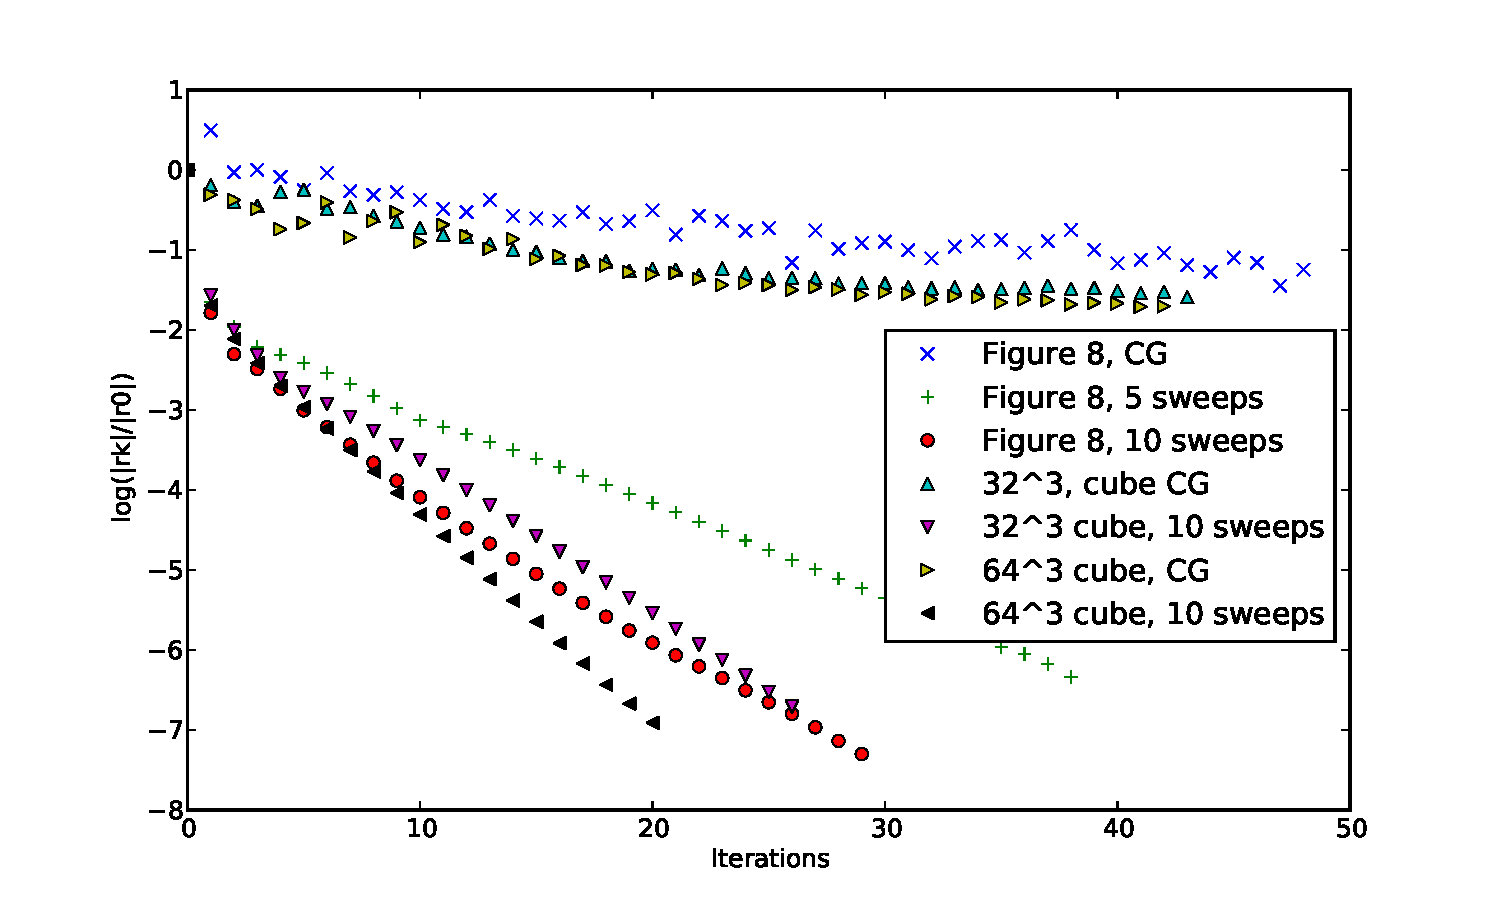
\includegraphics[width=.8\linewidth]{elasticity/figures/convergence_plot.pdf}}
\caption[Residual reduction $|r_k|_{\infty}/|r_0|_{\infty}$ per
  V-cycle or CG iteration for a number of examples.]{Residual reduction $|r_k|_{\infty}/|r_0|_{\infty}$ per
  V-cycle or CG iteration for a number of examples. In practice 1-3 v-cycles were necessary for each  Newton-Raphson update}
\label{fig:cube_convergence}
\end{figure}


We tested our full system on a number of production-quality models, focusing on regions where artists typically struggle to achieve realistic, collision-free results using traditional rigging methods.  

\subsection{Setup}
\begin{figure}[tb]
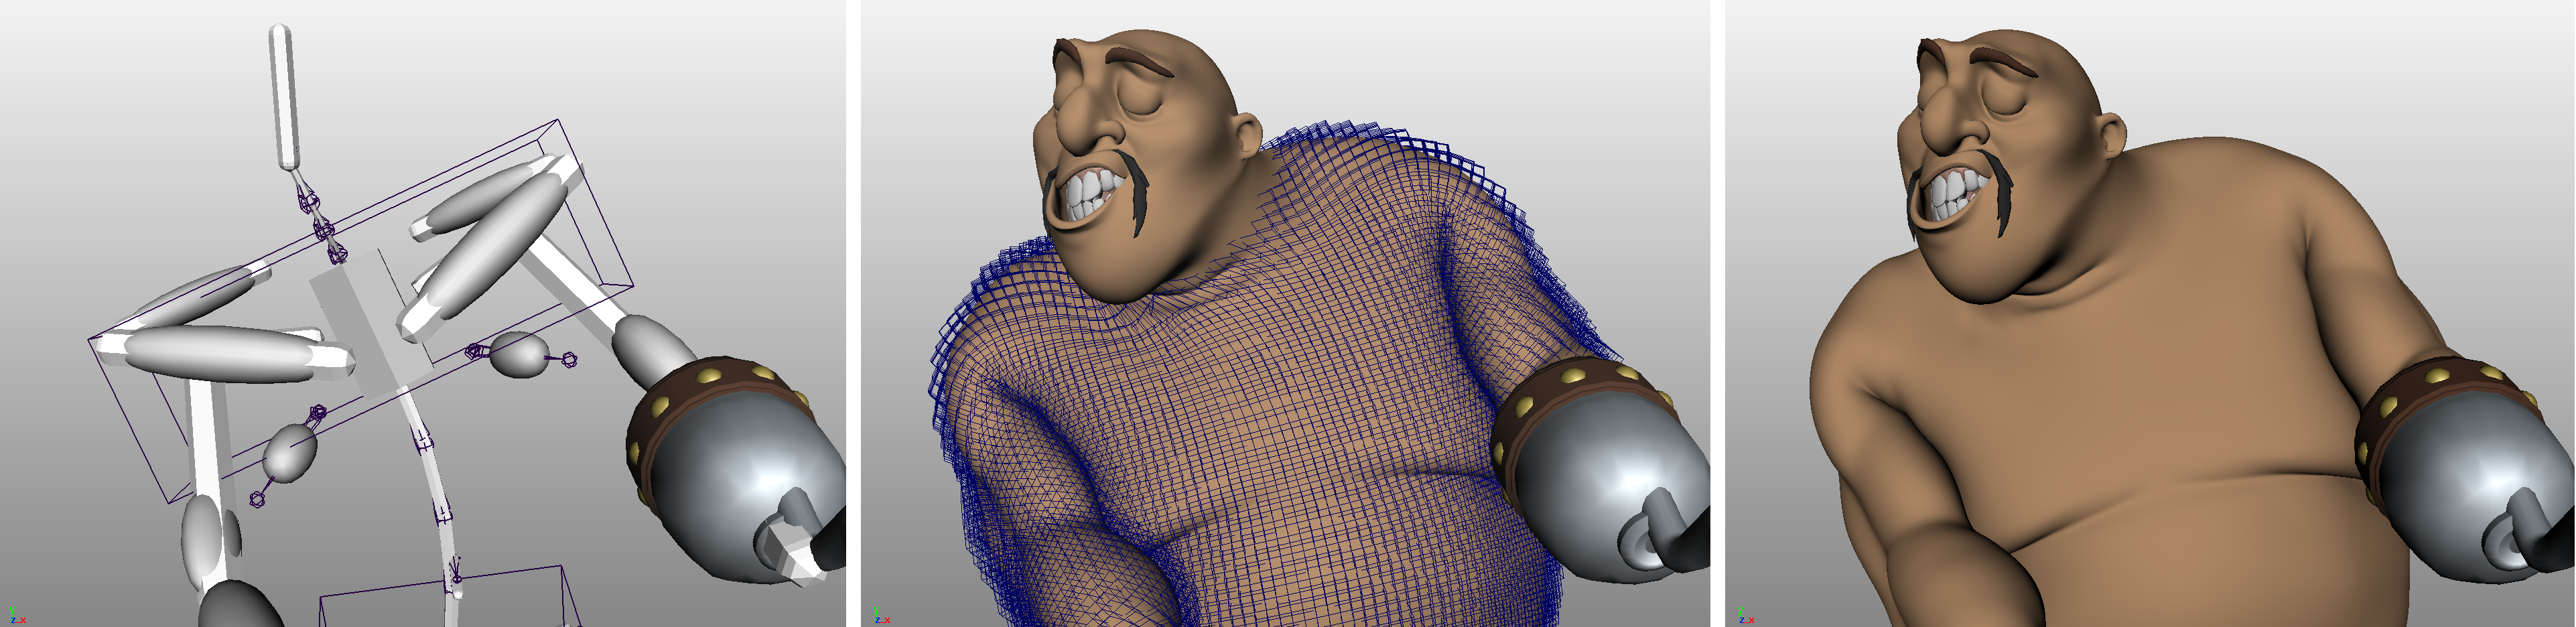
\includegraphics[width=\linewidth]{elasticity/figures/teaser3}
 \caption[The setup procedure for our method.]{Our method takes a geometric internal skeleton (left) and a source
   surface mesh (not pictured) as input. Based on a hexahedral lattice (center)
   it then simulates a deformed surface (right) obeying self-collision and volumetric
   elasticity. The example shown here has 106,567 cells and simulates at 5.5
   seconds per frame. Images \copyright Disney. All rights reserved.}\label{fig:teaser}
\end{figure}
Our simulation is driven by rigid bones attached to the character's existing skeleton.  Simple geometric shapes such as cylinders or ellipsoids are sufficient to define the volumetric extent of these bones, and we found that using soft constraints with narrow bones gave the elasticity model freedom to produce appealing flesh-like shapes. More carefully modeled bones can be used as internal collision objects over which the material can slide, providing detail in regions such as the elbow or around the collarbone. Finally, our self collision handling not only prevents interpenetration, it also works with our elastic simulation to create realistic squishing and bulging behavior.  

In addition to these basic features, in our examples we allow our deformer to be applied to sub-regions of the character mesh. Soft constraints ``stitch'' the simulation region to the underlying mesh in blend regions, allowing for a seamless transition.  

For highly stylized characters, detailed underlying structures such as muscles and tendons are often unclear or at least time consuming to create. By supporting spatially varying material parameters, we are able to easily approximate many of these coarse grain features.  Our interface allows users to paint material parameters onto the surface mesh; the parameters are then extrapolated to the volume by solving a Laplace equation.  Whereas we often attain acceptable results with constant material parameters, we can better sculpt shapes by varying the stiffness and Poisson's ratio of the material.

\subsection{Examples}
\begin{figure*}[tb]
\center{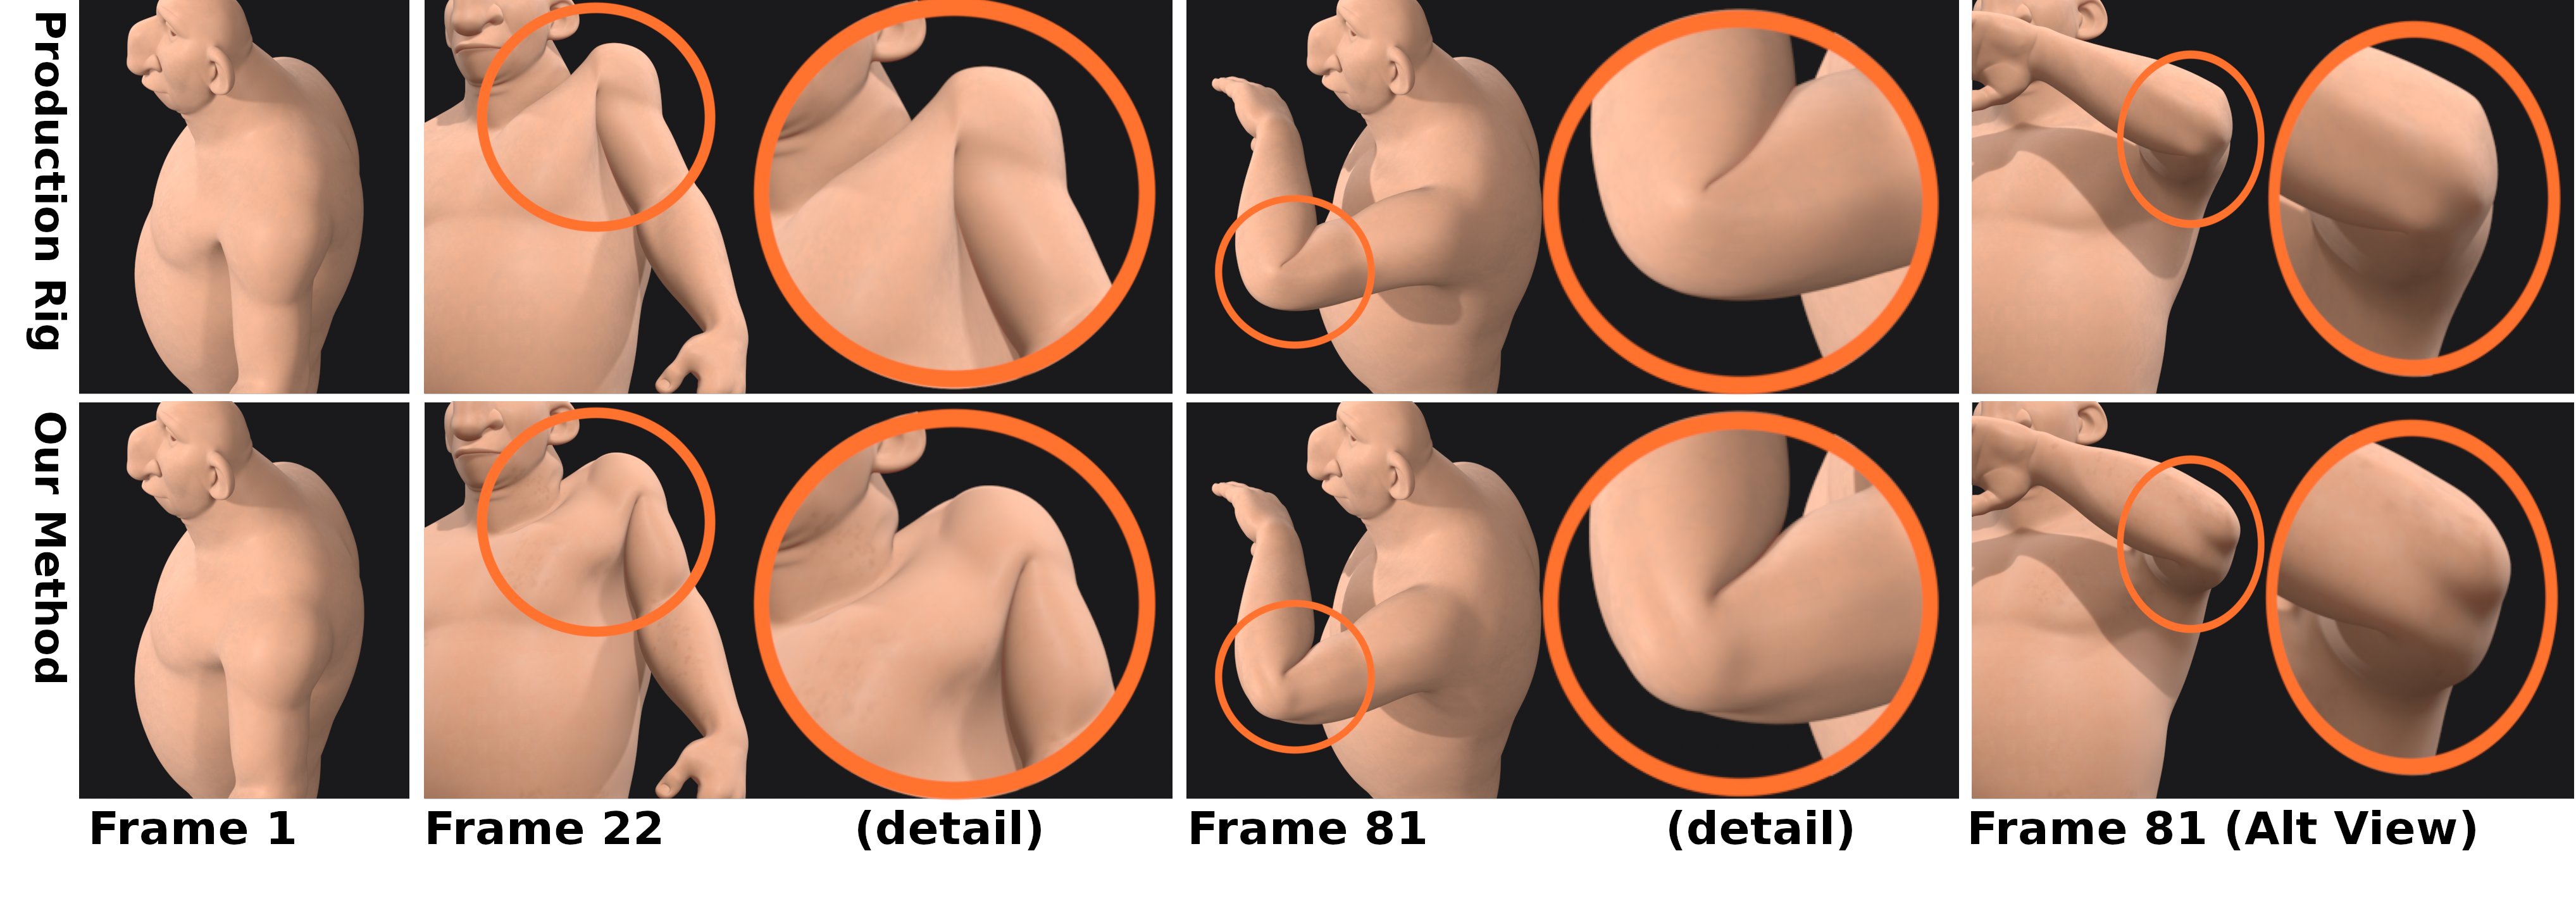
\includegraphics[width=\linewidth]{elasticity/figures/thugfigure}}
\caption[A comparison with linear blend skinning on a character arm
  and shoulder.]{A common problem with many existing techniques (and linear blend
  skinning in particular) is that it can be very difficult to maintain the
  illusion of an underlying bone-structure. As an example the top row here shows
  how the integrity of the region around the clavicle is lost as the character
  shrugs. In the bottom row, however, everything behaves as a connected
  entity. On the outside of the elbow we also get a nice protrusion of the ulna
  with our method as opposed to the more rubber-like behavior of the linear
  blend skin. The simulation here is based on 30,904 non-empty cells. Images \copyright Disney. All rights reserved.}
\label{fig:thug}
\end{figure*}
In all examples, we found that 1-2 V-cycles with 5 relaxation sweeps
per grid transfer were sufficient for the linear solver.  The number
of Newton iterations required depended on our initial guess; when
using the previous frame of an animation, we typically required
between 1 and 10 iterations for full convergence.  All reported CPU
times were computed on an 8-core Intel Xeon X5550 workstation.  GPU
tests were performed on an NVIDIA Quadro 6000. For interactive use it
should be noted that faster feedback can be provided by progressively
updating the display after each Newton iteration.

In Figure~\ref{fig:cube_convergence}, we compare convergence rates per
V-cycle or conjugate gradients iteration for a number of examples.  We
suspect that initial ``bump'' in residual reduction per V-cycle can be
explained by the efficiency of our Jacobi smoother.  We note that a
constant convergence rate emerges for all multigrid examples, in
contrast with CG.

In our first example, we applied our deformer to the arm, shoulder and neck region of a character (see Fig. \ref{fig:thug}). Each Newton iteration averaged 0.492s on the CPU and 0.345s on the GPU.  Our average frame times were 3.22s and 2.38s on the CPU and GPU respectively.

In Figure \ref{fig:hand}, we demonstrate our method on a character hand.  On the CPU, we averaged 1.40s per Newton iteration for an average of 12.6s per frame.  On the GPU, each Newton iteration averaged  0.612s for an average of 5.74s per frame.

Finally, in Figure~\ref{fig:teaser} we apply our deformer to the torso and arms of a large character with 106,567 elements. On the CPU, each Newton iteration was approximately 0.876s for a total of 5.48s per frame.  Our GPU implementation averaged 0.762s per Newton iteration and 5.14s per frame.


\section{Discussion}
\label{sec:discussion}
%##    * Shape richness improving artistic experience
%    * Speed as a game changer
%    * GPU versus CPU
%    * Future work : Physical parameters can still be unintuitive for artists.
%    * Future work : Art direction.

Originally, we were motivated by the desire to make true physically based
elasticity practical for production character rigging. We found that beyond our
expectations, artists were impressed with the shapes a physical deformer could
provide with little manual effort. What usually took days of weight
painting or pose example sculpting was now easy to achieve, and what was
impossible, collision and contact, was now possible.

A major decision in our project was to focus on optimizing for the CPU,
because we were familiar with CPU optimization and because
simulations often need to run on clusters without GPUs.  At the same
time we recognize GPUs are becoming more important because of their power and we
sought to experiment with the GPU. Though we have little experience with the
GPU, we believe our method will perform even better on the GPU with further
optimizations. Further, we note that most GPU experiments tend to compare
against relatively unoptimized CPU implementations, whereas our CPU
implementation was heavily optimized. Regardless we suspect that the GPU
implementation can still be improved significantly. 

Obviously, speed has been a major hurdle for the use of physical simulation in
production, so the fact that our simulations can run at near-interactive rates,
changes the game for artists. Even so, there is plenty of future work to do. One
area is making the parameters (like the Young's modulus) more intuitive for
artists to control, and another is allowing art direction in other ways, such as optimized
control (which also requires fast solvers). \newtext{Improvements to
the initial guess would improve robustness. Especially in the presence
of collisions. It would also allow more accurate self collision treatment in highly
deformed regions.  Finally, our solver
does not support near incompressible materials, and we would be
interested in exploring additional features such as material anisotropy.} But even without this future work, we
believe that our contribution will help create the next generation of appealing
characters. 

% In conclusion, we introduced a new stable corotated linear discretization that
% is robust, requires only one polar decomposition per cell, handles contact
% collision and constraints. We demonstrated a new polar decomposition algorithm
% that requires no trigonometric functions and is 40x faster than any other known
% implementation.  We implemented our new method on both the CPU and GPU and
% demonstrated its efficacy on several production quality examples.

